\documentclass[parskip=full,11pt]{scrartcl}

\usepackage[utf8]{inputenc}
\usepackage[T1]{fontenc}
\usepackage[german]{babel}

\usepackage[yyyymmdd]{datetime} % must be after babel
\renewcommand{\dateseparator}{-} % ISO8601 date format
\usepackage{hyperref}
\usepackage{listings}
\usepackage{float}
\usepackage{enumitem}
\renewcommand{\familydefault}{\sfdefault}
\usepackage{graphicx}
\usepackage{placeins}

\usepackage{lmodern}
\usepackage{courier}
\lstset{basicstyle=\footnotesize\ttfamily,breaklines=true}
\lstset{framextopmargin=50pt,frame=bottomline,showstringspaces=false}


\RedeclareSectionCommand[style=section,indent=0pt,font=\usekomafont{partnumber}]{part}
\renewcommand*{\partformat}{\thepart\enskip}

\RedeclareSectionCommand[beforeskip=0pt ,afterskip=0pt]{subparagraph}

\usepackage[bottom = 3 cm, top = 3 cm]{geometry}

% command for an attribute
\newcommand{\attr}[4]{\lstinline{[#3]} \textbf{\lstinline{#1 : #2}} \newline #4}

% command for a method
\newcommand{\method}[5]{\lstinline{[#4]} \textbf{\lstinline{#1 (#3) : #2}} \newline #5}

% command for a constructor
\newcommand{\ctor}[4]{\lstinline{[#3]} \textbf{\lstinline{#1 (#2)}} \newline #4}

	\begin{document}
	\title{Entwurf: Programmanalyse zum Durchklicken}
	\author{Nils Jessen \and Anika Nietzer \and Patrick Petrovic \and Sebastian Rauch \and Michael Schieber}
	
	\maketitle
	
	
	\part{Entwurfsentscheidungen}

\section{Einleitung}
Dieses Dokument beschreibt den Entwurf des Programms "Datenflussanalyse zum Durchklicken". Es ist nach dem Top-Down-Prinzip aufgebaut. 
Zunächst werden in diesem einführenden Abschnitt unsere Entwurfsentscheidungen beschrieben und die Beweggründe, auf welchen diese beruhen, näher erläutert.
Es wird eine Übersicht über alle Pakete gegeben und die Aufgaben der verwendeten externen Libraries werden beschrieben. 
Anschließend folgt eine detaillierte Beschreibung aller Klassen und die Erklärung aller öffentlichen Methoden. 
Wichtige private Attribute werden genannt, um die Vollständigkeit zu gewährleisten und um die Funktionen öffentlicher Methoden zusammenhängend erklären zu können. 
Im Anschluss werden Sequenzdiagramme der wichtigsten Funktionen des Programms gezeigt, Änderungen in Bezug auf das Pflichtenheft aufgelistet und ein vollständiges Klassendiagramm aller Klassen angehängt.

\section{Architektur}
Bei diesem Entwurf wird das Model-View-Controller (MVC) Architekturmuster verwendet. 
Diese Entwurfsentscheidung erleichtert die spätere Weiterentwicklung und die Erweiterung des Programms mit weiterer Funktionalität. \par
Das Modell dieser Architektur beinhaltet die darzustellenden Daten und die erforderliche Logik für die Funktionalität des Programms. 
Die Präsentationsschicht beinhaltet die für die Darstellung und die Interaktion mit dem Benutzer notwendigen Daten. Die Steuerung ist für die Umsetzung der vom Benutzer geforderten Änderungen/Funktionalität zuständig. 
Sie wird durch die Benutzerinteraktion angesprochen und informiert das Modell über die zu ändernden Daten oder notwendigen Vorgänge.

\section{Modulübersicht}
Der Entwurf setzt sich aus den in der folgenden Graphik dargestellten Modulen gemäß dem MVC-Muster zusammen.
Dabei gehören das DFAFramework-Modul, das Analysen-Modul, das CodeProcessor-Modul und das Reflections-Modul zum Model. 
Der View wird durch das GUI-Modul, das VisualGraph-Modul und das JGraphX-Modul gebildet. \par
Das DFAFramework liefert die Logik für die Funktionalität des Programms. 
Es benutzt dabei das Analyse-Modul, in welchem sich die von uns implementierten Datenflussanalysen befinden. 
Diese Datenflussanalysen implementieren ein zentrales Interface des DFAFrameworks. 
Des Weiteren ist es abhängig von den externen Libraries Soot und Reflections (siehe unten). 
Der Controller ist für die Kommunikation zwischen dem DFAFramework und dem User Interface zuständig. 
Dabei benutzt er das InputProcessor-Modul, welches zwischen dem Controller und Soot vermittelt. 
Durch diesen Input-Prozessor ist der Controller weitestgehend unabhängig von der verwendeten Library Soot. \par 
Das GUI-Modul ist für die Darstellung der Information und für die Interaktion mit dem Benutzer zuständig. 
Dabei verwendet es das VisualGraph-Modul, welches für die Kommunikation zwischen der logischen Struktur des DFAFrameworks und der visuellen Information im \inlinecode{VisualGraphPanel} inklusive der Interaktion des Benutzers mit diesem verantwortlich ist. 
Das VisualGraph-Modul verwendet die Libary JGraphX und ist ebenfalls für den Export von Graphen verantwortlich.

\begin{figure}[htbp] 
  \centering
     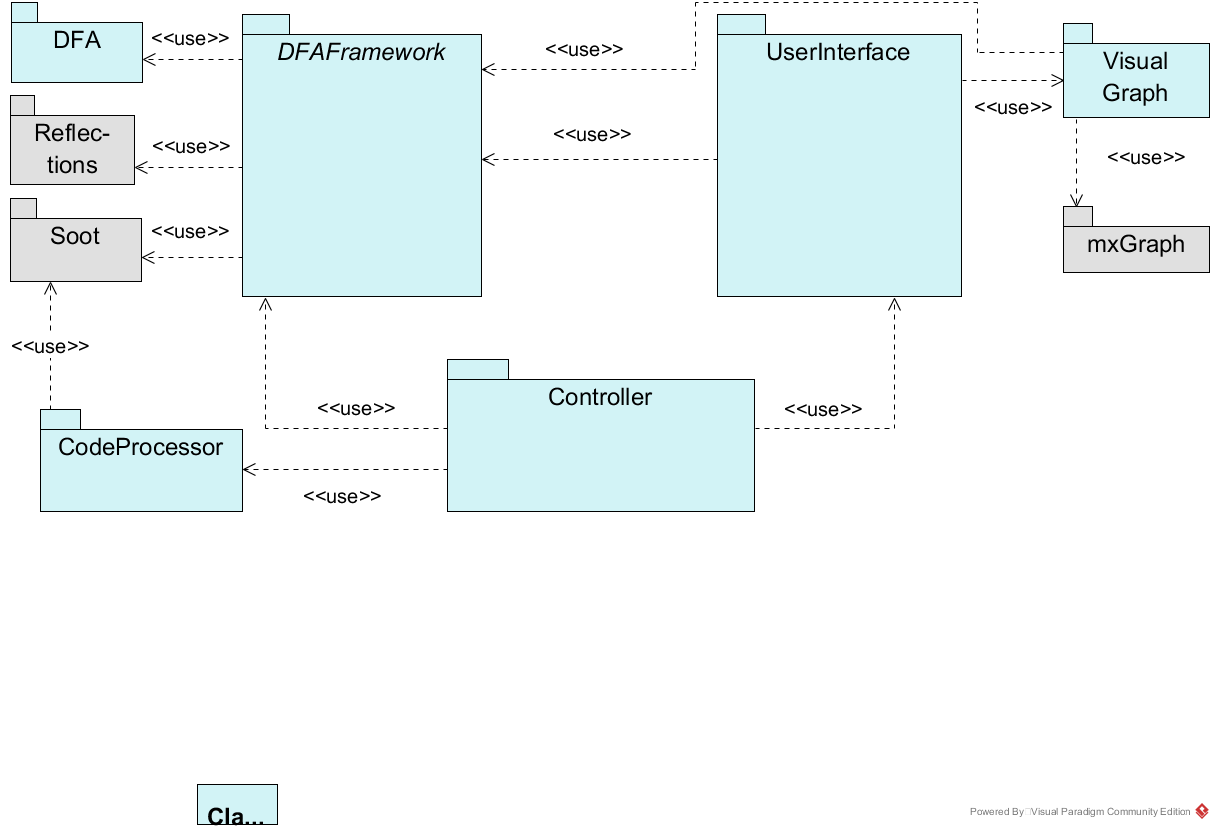
\includegraphics[width=1\textwidth]{Entwurfsentscheidungen/PackageOverview}
  \caption{Modulübersicht}
  \label{fig:Ubersicht}
\end{figure}

\newpage
\section{Externe Libraries}

\subsection{JGraphX}

JGraphX (\url{https://github.com/jgraph/jgraphx}) ist eine Java-Library zum automatischen Layouten und zum Zeichnen von Graphen. 
Damit eignet sich JGraphX gut, um den im Rahmen der Animation von Datenflussanalysen erstellten Kontrollflussgraphen zu visualisieren. Insbesondere bietet JGraphX die Möglichkeit, Knoten weiter in Zellen (\lstinline{mxCell}) zu unterteilen.
Dies ermöglicht die zeilenweise Animation der Datenflussanalysen.

\subsection{Reflections}

Reflections (\url{https://github.com/ronmamo/reflections}) ist eine Java-Library, die es erlaubt, zur Laufzeit neue Java-Klassen zu laden, sowie Metainformation über diese zu erhalten.
Dies wird dazu benutzt, um zur Laufzeit neue Datenflussanalysen zu laden.
Dazu wird ein festgelegter Ordner bei Programmstart auf kompilierte Java-Dateien (.class-Dateien) aus einem bestimmten Package [?! noch festlegen !?] untersucht. 
Dann werden alle Klassen, die von \lstinline{DataFlowExecution} erben, geladen und als Datenflussanalysen bereitgestellt. 


\subsection{Soot}

Soot (\url{https://github.com/Sable/soot}) ist eine Java-Library, die viele Funktionalitäten für statische Programmanalysen bereitstellt. 
Insbesondere bietet Soot mehrere Zwischencode-Formate an, in die gegebener Java-Bytecode übersetzt werden kann. 
In diesem Projekt wird Jimple als Zwischencode verwendet, auf dem die Datenflussanalysen erfolgen.
Bei Jimple handelt es sich um einen Expression-basierten typisierten Drei-Adress-Code.
Die elementaren Codeeinheiten sind also Expressions (Ausdrücke), die jeweils maximal drei Operanden haben.
Neben einer Zwischencode-Repräsentation bietet Soot die Möglichkeit, einen Kontrollflussgraphen aus Java-Bytecode zu erzeugen.
Die Grundblöcke des erzeugten Kontrollflussgraphen enthalten dann entsprechenden Zwischencode (hier Jimple).
	
	%note: don't split this document up with include{...}

\part{Klassenbeschreibung}

% the template for one class description

%\class{SomeClass extends Watever implements DontCare}
%Brief descrition of SomeClass.

%\subparagraph{Attribute} % skip this if there are no attributes
%\begin{itemize}
%	\item \attr{attrName}{type}{visibility}{
%		Description of the attribute.
%	}
%\end{itemize}
%
%
%\subparagraph{Konstruktoren} % skip this if there are no constructors
%\begin{itemize}
%	\item \method{constructorName}{type}{paramList}{visibility}{
%		Description of the constructor.
%	}
%\end{itemize}
%
%\subparagraph{Methoden}  % skip this if there are no methods
%\begin{itemize}
%	\item \method{methodName}{type}{paramList}{visibility}{
%		Description of the method.
%	}
%\end{itemize}
	%note: don't split this document up with include{...}

\section{Controller}

\subsection{Klassendiagramm}

\begin{figure}[htbp] 
  \centering
  		 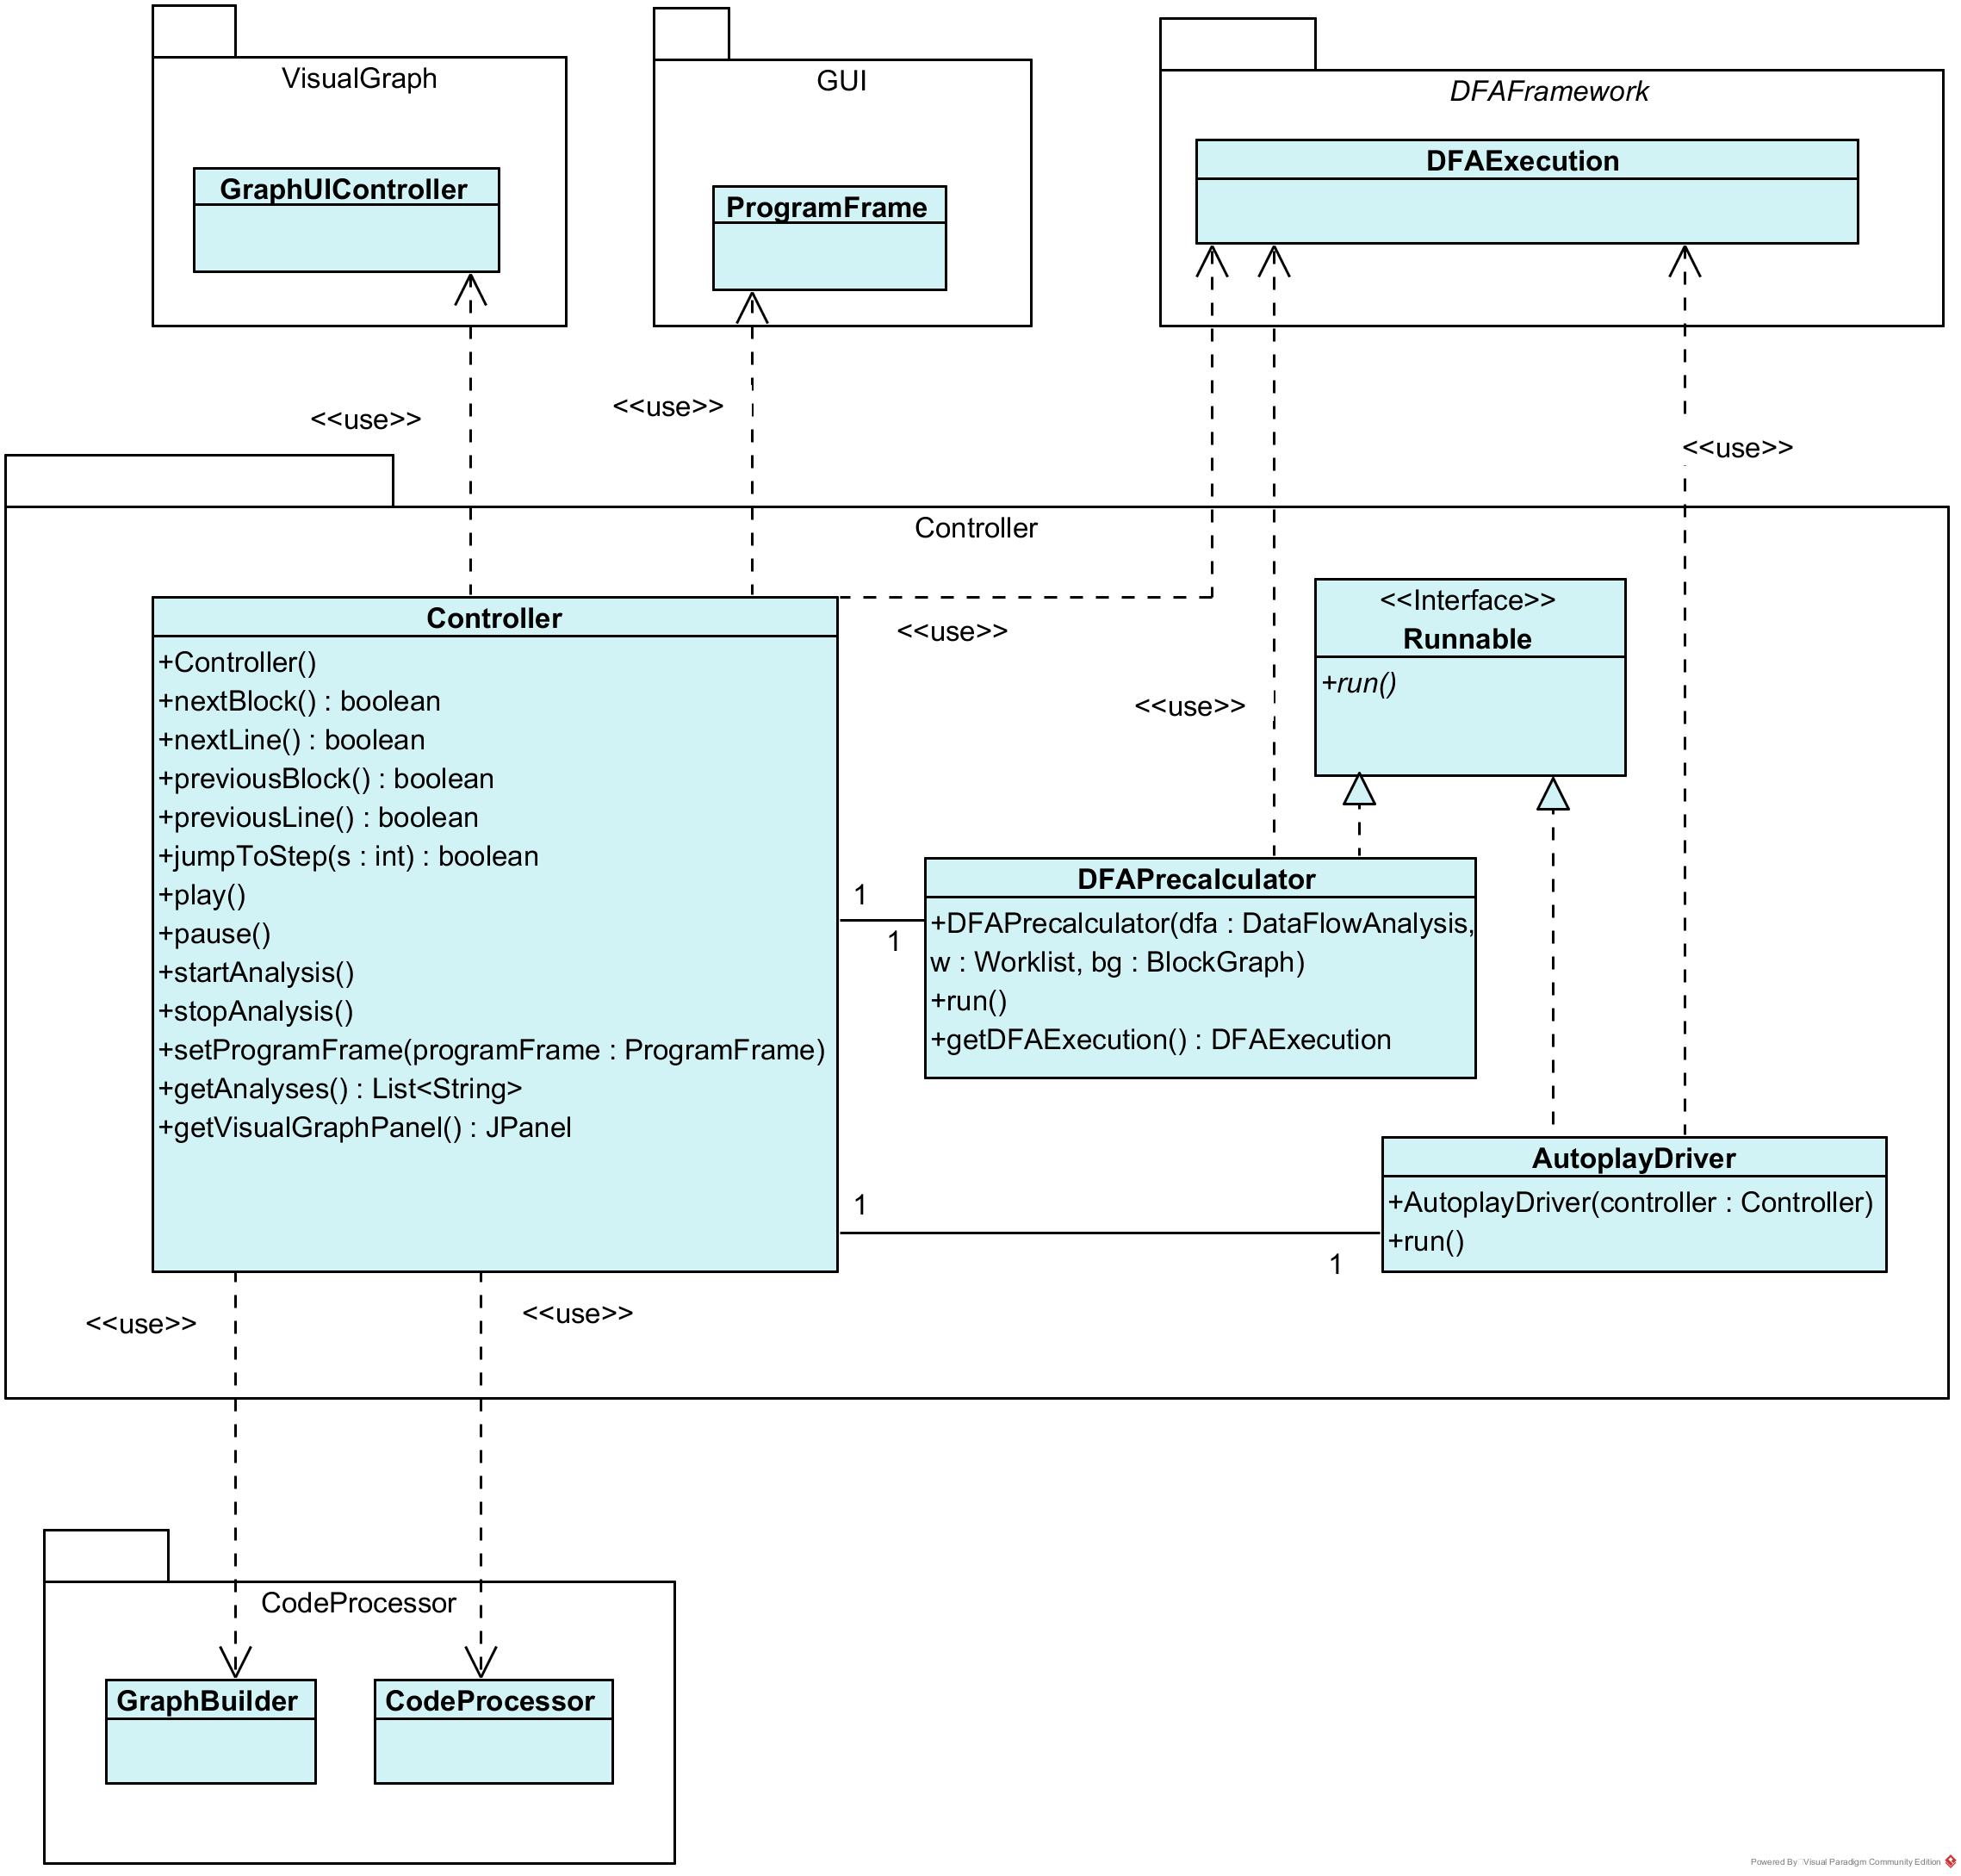
\includegraphics[width=1\textwidth]{Klassenuebersicht/Controller/Controller}
  \caption{Klassendiagramm des User Interfaces}
  \label{fig:UI}
\end{figure}

\subsection{Modulbeschreibung}

Das Controller-Modul ist dafür verantwortlich, die Kommunikation zwischen der Graphischen Benutzeroberfläche (\inlinecode{GUI}) und dem Datenflussanalyse-Framework (DFAFramework) sowie dem CodeProcessor-Modul zu übernehmen.
Außerdem bietet es eine Schnittstelle zum VisualGraph-Modul.

Die Grundidee des \inlinecode{Controllers} basiert auf dem Model-View-Controller Muster (MVC).

Der \inlinecode{Controller} wird benutzt sobald der Benutzer ein GUI-Element benutzt, welches eine Veränderung des Models (\inlinecode{DFAFramework}) nach sich ziehen muss. Darunter fällt zum Beispiel das Starten der Analyse oder die Steuerung der Analyseschritte.
Nicht darunter fällt eine reine Änderung der GUI-Anzeige, wie beispielsweise das Ändern der Größe des Fensters.

Wird nun beispielsweise eine neue Analyse gestartet, so wird der \inlinecode{Controller} von der GUI aufgerufen und beschafft sich alle nötigen Informationen von der GUI.
Dann lässt er den \inlinecode{CodeProcessor} den zu analysierenden Code in einen Kontrollflussgraphen umbauen und gibt diesen dann dem DFAFramework. Dieses berechnet dann die Datenflussanalyse.
Sobald dies abgeschlossen ist, lässt der \inlinecode{Controller} die GUI aktualisieren, wobei er auf dem \inlinecode{GraphUIController} die \inlinecode{start()}-Methode aufruft.
Diese sorgt dafür, dass der Benutzer den Graph im \inlinecode{VisualGraphPanel} sehen kann. Alle anderen Panels steuert der \inlinecode{Controller} selbst an.

Während der Analyse wird der \inlinecode{Controller} weiterhin von der GUI aufgerufen, um die Analyse zu steuern. Der Controller lässt dabei immer das DFAFramework aktualisieren und dann die \inlinecode{GUI} die neuen Informationen anzeigen.

Bei Aktionen die möglicherweise viel Zeit benötigen, erzeugt der \inlinecode{Controller} einen neuen \inlinecode{Thread} um diese Aktion abzuarbeiten.
Dadurch soll die Reaktionsfähigkeit des Programms garantiert werden.

Für den Entwurf ergeben sich folgende Vorteile:
\begin{itemize}
	\item Durch den \inlinecode{Controller} ist die Anwendungslogik klar von den Darstellungen und Benutzerinteraktionen getrennt.
	Dadurch kann die Benutzeroberfläche leicht ausgetauscht werden.
	\item Der Status der Datenflussanalyse kann leicht in unterschiedlichen Darstellungsmodulen repräsentiert werden, wie zum Beispiel als Graph (\inlinecode{VisualGraphPanel}) und als Status eines Knotens (\inlinecode{StatePanel}).
	\item Das bestehende System kann leicht erweitert werden indem neue Teile zum Model (DFAFramework) oder View (GUI) hinzugefügt werden.
\end{itemize}

% the template for one class description
\subsection{Klassenbeschreibung}

\class{Controller}

%Brief descrition of SomeClass.
Die Klasse \inlinecode{Controller} ist für den Großteil der Kommunikation zwischen der GUI und den restlichen Modulen des Programmes zuständig.

\paragraph{Konstruktoren} % skip this if there are no constructors
\begin{itemize}
	\item \ctor{Controller}{}{public}{
		Erzeugt einen \inlinecode{AnalysisLoader} und lädt Analysearten.
		Außerdem wird der \inlinecode{GraphUIController} erzeugt.
	}
\end{itemize}

\paragraph{Methoden}  % skip this if there are no methods
\begin{itemize}
	\item \method{nextBlock}{boolean}{}{public}{
		Wird aufgerufen, sobald in der GUI das entsprechende Event ausgelöst wurde.
		Lässt das DFAFramework den nächsten Block (Knoten des Kontrollflussgraphen) berechnen und sorgt dann dafür, dass der \inlinecode{GraphUIController} das \inlinecode{VisualGraphPanel} aktualisiert.
		
		Gibt \inlinecode{true} zurück, falls dies erfolgreich war, \inlinecode{false} wenn nicht.
	}
	\item \method{nextLine}{boolean}{}{public}{
		Wird aufgerufen, sobald in der GUI das entsprechende Event ausgelöst wurde.
		Lässt das DFAFramework die nächste Zeile innerhalb eines Blocks berechnen, oder springt zum nächsten Block. Danach sorgt er dafür, dass der \inlinecode{GraphUIController} das \inlinecode{VisualGraphPanel} aktualisiert.
		
		Gibt \inlinecode{true} zurück, falls dies erfolgreich war, \inlinecode{false} wenn nicht.
	}
	\item \method{previousBlock}{boolean}{}{public}{
		Wird aufgerufen, sobald in der GUI das entsprechende Event ausgelöst wurde.
		Lässt das DFAFramework den vorherigen Block (Knoten des Kontrollflussgraphen) berechnen und sorgt dann dafür, dass der \inlinecode{GraphUIController} das \inlinecode{VisualGraphPanel} aktualisiert.
		
		Gibt \inlinecode{true} zurück, falls dies erfolgreich war, \inlinecode{false} wenn nicht.
	}
	\item \method{previousLine}{boolean}{}{public}{
		Wird aufgerufen, sobald in der GUI das entsprechende Event ausgelöst wurde.
		Lässt das DFAFramework die vorherige Zeile innerhalb eines Blocks berechnen, oder springt zum Anfang dieses Blocks. Danach sorgt er dafür, dass der \inlinecode{GraphUIController} das \inlinecode{VisualGraphPanel} aktualisiert.
		
		Gibt \inlinecode{true} zurück, falls dies erfolgreich war, \inlinecode{false} wenn nicht.
	}
	\item \method{jumpToStep}{boolean}{s : int}{public}{
		Wird aufgerufen, sobald in der GUI das entsprechende Event ausgelöst wurde.
		Lässt das DFAFramework eine bestimmte Zeile oder einen bestimmten Block berechnen und sorgt dann dafür, dass der \inlinecode{GraphUIController} das \inlinecode{VisualGraphPanel} aktualisiert.
		
		Gibt \inlinecode{true} zurück, falls dies erfolgreich war, \inlinecode{false} wenn nicht.
	}
	\item \method{play}{void}{}{public}{
		Wird aufgerufen, sobald in der GUI das entsprechende Event ausgelöst wurde.
		
		Erzeugt einen \inlinecode{AutoplayDriver}, welcher ein \inlinecode{Thread} ist, der die Schritte der Datenflussanalyse automatisch durchgeht.
		Dies passiert durch mehrmaliges aufrufen der \inlinecode{nextLine()}-Methode (bei eingestelltem Delay größer als 0 Sekunden).
		
		Ruft \inlinecode{jumpToStep()} mit dem letzten Schritt der Analyse auf, falls der Delay auf 0 Sekunden eingestellt ist.
	}
	\item \method{pause}{void}{}{public}{
		Wird aufgerufen, sobald in der GUI das entsprechende Event ausgelöst wurde. 
		Unterbricht den \inlinecode{AutoplayDriver}, sodass der Benutzer wieder manuell alle Schritte durchgehen kann.
		
	}
	\item \method{startAnalysis}{void}{}{public}{
		Wird aufgerufen, sobald in der GUI das entsprechende Event ausgelöst wurde.
		Beschafft sich alle nötigen Informationen von der GUI.
		Lässt dann die \inlinecode{CodeProcessor}-Klasse aus der Benutzereingabe Java-Bytecode kompilieren.
		Dieser wird vom \inlinecode{GraphBuilder} in einen \inlinecode{BlockGraph} umgewandelt und dem  \inlinecode{DFAPrecalculator} zusammen mit einer \inlinecode{Worklist} und einer \inlinecode{DataFlowAnalysis} übergeben, um den Kontrollflussgraphen und die Schritte der Datenflussanalyse vor zu berechnen. Danach wird auf dem \inlinecode{GraphUIController} \inlinecode{start()} aufgerufen, um den Kontrollflussgraphen anzeigen zu lassen.
		
		In der GUI werden das \inlinecode{StatePanel}, das \inlinecode{ControlPanel} und das \inlinecode{VisualGraphPanel} aktiviert. Das \inlinecode{InputPanel} wird deaktiviert.
	}
	\item \method{stopAnalysis}{void}{}{public}{
		Wird aufgerufen sobald in der GUI das entsprechende Event ausgelöst wurde.
		Verwirft die aktuelle \inlinecode{DFAExecution} und lässt den \inlinecode{GraphUIController} den Inhalt des \inlinecode{VisualGraphPanels} löschen.
		Abschließend werden  das \inlinecode{ControlPanel}, das \inlinecode{StatePanel} und das \inlinecode{VisualGraphPanel} deaktiviert und das \inlinecode{InputPanel} aktiviert. 
		
	}
	\item \method{setProgramFrame}{void}{programFrame : ProgramFrame}{public}{
		Übergibt dem \inlinecode{Controller} das \inlinecode{ProgramFrame}.
		Dieser kann darüber auf die GUI-Elemente zugreifen.
	}
	\item \method{getAnalyses}{List<String>}{}{public}{
		Gibt eine Liste mit den Namen der Analysen zurück, welche beim Programmstart vom \inlinecode{AnalysisLoader} gefunden wurden.
	}
	\item \method{getVisualGraphPanel}{JPanel}{}{public}{
		Gibt das \inlinecode{VisualGraphPanel}, welches der \inlinecode{GraphUIController} erstellt hat zurück.
	}
\end{itemize}

\subsubsection{DFAPrecalculator implements Runnable}
%Brief descrition of SomeClass.
Diese Klasse lässt die \inlinecode{DFAExecution} die Datenflussanalyse in einem separaten \inlinecode{Thread} vorberechnen, sodass der Benutzer die Berechnung abbrechen kann falls sie in eine Endlosschleife läuft oder zu viel Speicher verbraucht.


\subparagraph{Konstruktoren} % skip this if there are no constructors
\begin{itemize}
	\item \ctor{DFAPrecalculator}{dfa : DataFlowAnalysis, w : Worklist, bg : Blockgraph}{public}{
		Übergibt dem \inlinecode{DFAPrecalculator} alle nötigen Daten um eine \inlinecode{DFAExecution} zu erzeugen.
	}
\end{itemize}

\subparagraph{Methoden}  % skip this if there are no methods
\begin{itemize}
	\item \method{run}{void}{}{public}{
		Wird beim Starten des \inlinecode{Threads} aufgerufen und lässt die \inlinecode{DFAExecution} vorberechnen.
	}
	
	\item \method{getDFAExecution}{dfae : DFAExecution}{}{public}	{
	Gibt die berechnete \inlinecode{DFAExecution} zurück.
	}
\end{itemize}

\class{AutoplayDriver implements Runnable}
%Brief descrition of SomeClass.
Diese Klasse lässt die einzelnen Schritte der Analyse ablaufen, wenn der Benutzer die Autoplay-Funktion benutzt. Sie arbeitet in einem separaten \inlinecode{Thread}.


\subparagraph{Konstruktoren} % skip this if there are no constructors
\begin{itemize}
	\item \ctor{AutoplayDriver}{controller : Controller}{public}{
		Übergibt dem \inlinecode{AutoplayDriver} eine Instanz der \inlinecode{Controller} Klasse, über welche sie die Schritte der Datenflussanalyse ausführen kann.
	}
\end{itemize}

\subparagraph{Methoden}  % skip this if there are no methods
\begin{itemize}
	\item \method{run}{void}{}{public}{
		Wird beim Starten des \inlinecode{Threads} aufgerufen und lässt die einzelnen Schritte der Analyse abarbeiten.
	}
\end{itemize}
	%note: don't split this document up with include{...}

\subsection{CodeProcessor}
	%note: don't split this document up with include{...}

\section{DFAFramework}

\subsection{Klassendiagramm}
\begin{figure}[htbp] 
	\centering
	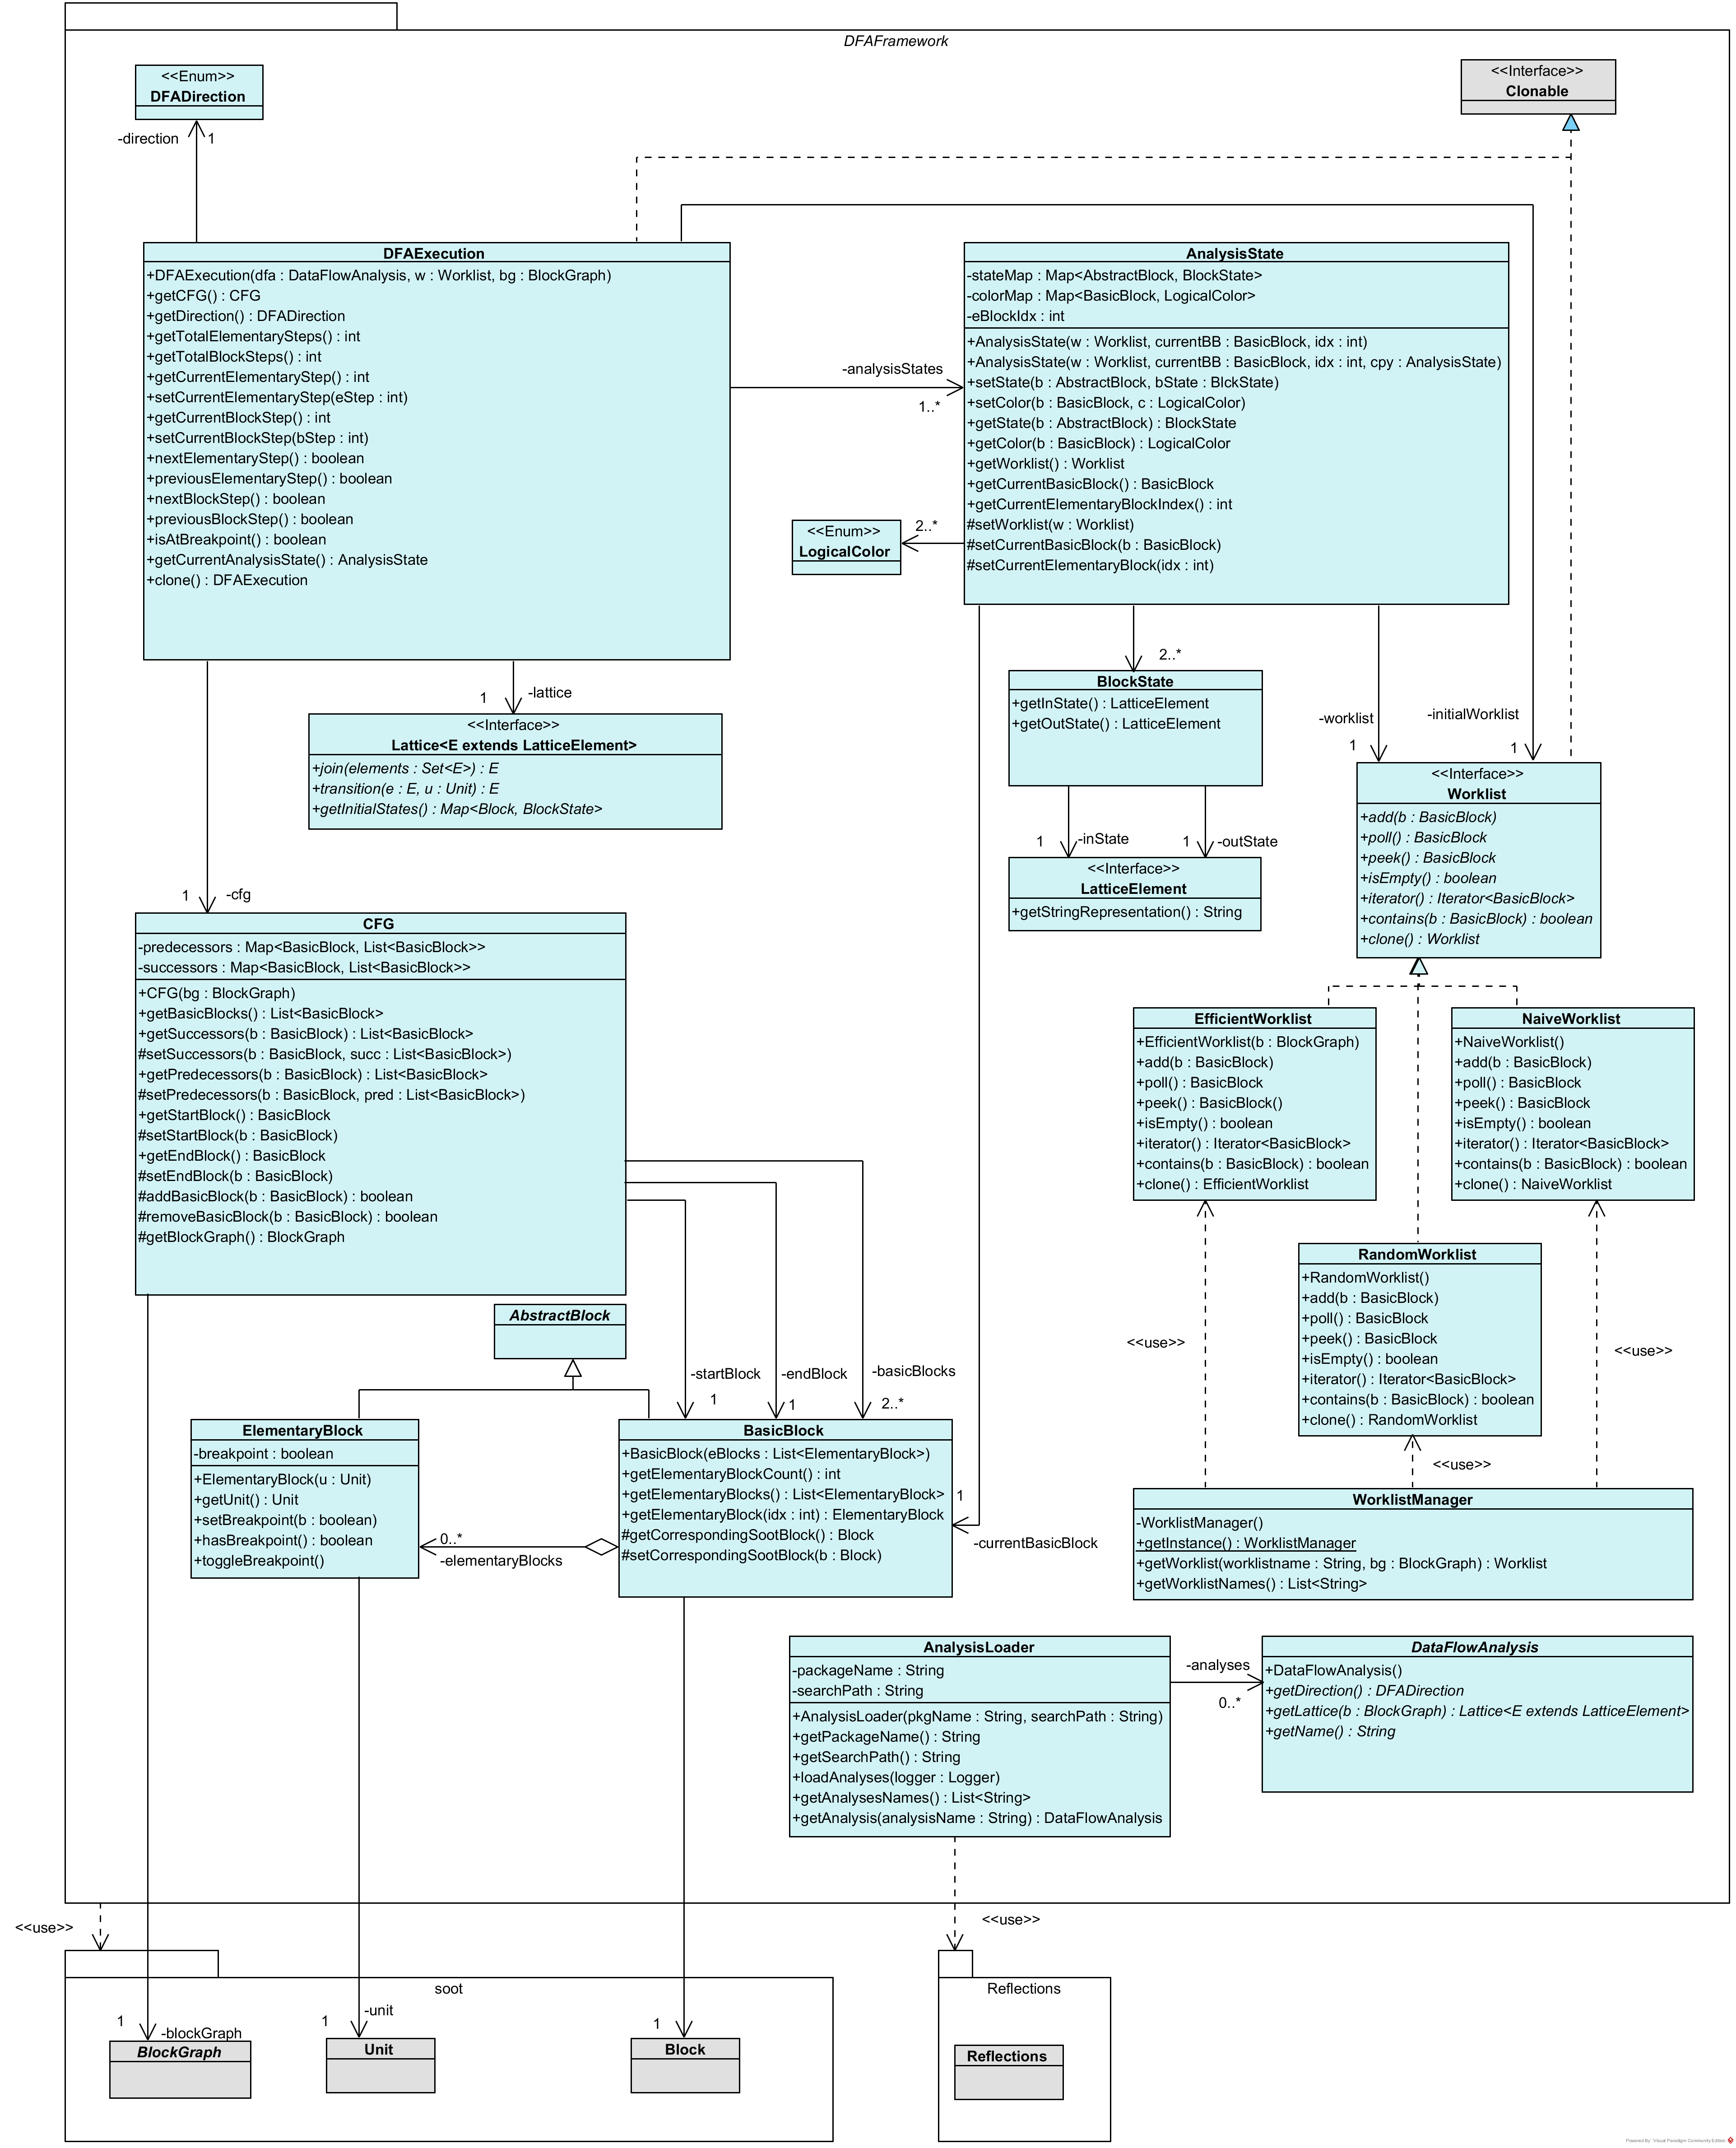
\includegraphics[width=1\textwidth]{Klassenuebersicht/DFAFramework/DFAFramework}
	\caption{Klassendiagramm des DFAFramework}
	\label{fig:DFAFreamework}
\end{figure}

%\newpage

Das DFAFramework ist für die Ausführung von Datenflussanalysen zuständig.
Weiter übernimmt das DFAFramework das Laden von Datenflussanalysen von einem festgelegten Speicherort.

Für die Ausführung von Datenflussanalysen ist die Klasse \inlinecode{DFAExecution} zentral.
Diese kann eine Datenflussanalyse für ein gegebenes \inlinecode{DataFlowAnalysis}-Objekt und einen gegebenen \inlinecode{BlockGraph} (\inlinecode{soot.toolkits.graph.BlockGraph}) vorberechnen.
Nach der Vorberechnung kann dann der aktuelle Analyseschritt mittels \inlinecode{nextElementaryStep()}, \inlinecode{previousElementaryStep()}, \inlinecode{setCurrentElementaryStep(stepNum : int)} und \inlinecode{getCurrentElementaryStep() : int} zeilenweise beliebig eingestellt bzw. abgefragt werden. 
Analog zu zeilenweisen Schritten können auch blockweise Schritte mittels \inlinecode{nextBlockStep()}, \inlinecode{previousBlockStep()}, \inlinecode{setCurrentBlockStep(step : int)} und \inlinecode{getCurrentBlockStep() : int} eingestellt und abgefragt werden.
Zudem kann mit \inlinecode{getCurrentAnalysisState() : AnalysisState} zu jedem Zeitpunkt der aktuelle Analysezustand erfragt werden.
Ein \inlinecode{AnalysisState} speichert dabei für jeden \inlinecode{AbstractBlock} (also sowohl für \inlinecode{ElementaryBlock}s als auch \inlinecode{BasicBlock}s) den aktuellen In- und Out-State, den aktuellen Zustand der \inlinecode{Worklist} sowie bei welchem \inlinecode{ElementaryBlock} bzw. \inlinecode{BasicBlock} sich die Analyse aktuell befindet.

Das Interface \inlinecode{Worklist} sowie die implementierenden Klassen \inlinecode{EfficientWorklist}, \inlinecode{NaiveWorklist} und \inlinecode{RandomWorklist} legen die Analysereihenfolge der einzelnen \inlinecode{BasicBlock}s fest und setzen damit das Entwurfsmuster der Strategie um.

Für die Implementierung konkreter Datenflussanalysen ist die Klasse \inlinecode{DataFlowAnalysis} essentiell.
Sie legt die Analyserichtung (\inlinecode{DFADirection}) sowie den Namen, unter dem eine Datenflussanalyse in der GUI auftaucht, fest.
Weiter bestimmt eine \inlinecode{DataFlowAnalysis} mittels \inlinecode{getLattice(blockGraph : BlockGraph) : Lattice} den für die Analyse verwendeten Verband.
Ein \inlinecode{Lattice} realisiert den Join-Operator mittels \inlinecode{join(elements : Set<LatticeElement>) : LatticeElement}.
Weiter gibt er zu allen unterstützten Expressions eine Übergangsfunktion mittels \inlinecode{transition(in : LatticeElement, unit : soot.Unit) : LatticeElement} an.
Schließlich gibt ein \inlinecode{Lattice} zu jedem Grundblock mittels \inlinecode{getInitialStates() : Map<Block, BlockState>} einen Initialzustand an. 
Mit den verschiedenen Implementierungen des Interfaces \inlinecode{Lattice} und den damit verbundenen Algorithmen für \inlinecode{join(elements : Set<LatticeElement>) : LatticeElement} und \inlinecode{transition(in : LatticeElement, unit : soot.Unit) : LatticeElement} kommt auch hier das Entwurfsmuster der Strategie fulminant zur Anwendung.

Ein \inlinecode{AnalysisLoader} ist für das Laden von Datenflussanalysen zuständig.
Mittels \inlinecode{loadAnalyses(logger : java.util.logging.Logger)} werden alle Unterklassen von \inlinecode{DataFlowAnalysis}, die an einem festgelegten Speicherort als .class-Dateien abgelegt sind, geladen.
Die Namen der geladenen Analysen können dann mit \inlinecode{getAnalysesNames() : List<String>} abgefragt werden.
Weiter kann mit \inlinecode{getAnalysis(analysisName : String) : DataFlowAnalysis} ein \inlinecode{DataFlowAnalysis}-Objekt über seinen Namen ermittelt werden.

\newpage

\subsection{Klassenbeschreibung}

\class{abstract DataFlowAnalysis}
\inlinecode{DataFlowAnalysis} ist die abstrakte Basisklasse für alle konkreten Datenflussanalysen.
Jede \inlinecode{DataFlowAnalysis} legt ihren Namen, die Richtung der Analyse sowie den verwendeten Verband fest.

\paragraph*{Konstruktoren} 
\begin{itemize}
	\item \ctor{DataFlowAnalysis}{}{public}{
	Instanziiert eine \inlinecode{DataFlowAnalysis}.
	}
\end{itemize}

\paragraph*{Methoden}
\begin{itemize}
	\item \method{getDirection}{DFADirection}{}{public abstract}{
	Gibt die \inlinecode{DFADirection} der \inlinecode{DataFlowAnalysis} zurück.
	}
	\item \method{getLattice}{Lattice<E extends LatticeElement>}{b : BlockGraph}{public abstract}{
	Gibt den \inlinecode{Lattice} zurück, auf welchem die \inlinecode{DataFlowAnalysis} basiert.
	}
	\item \method{getName}{String}{}{public abstract}{
	Gibt den Namen der \inlinecode{DataFlowAnalysis} zurück.
	}
\end{itemize}

\class{AnalysisLoader}
Ein \inlinecode{AnalysisLoader} ist für das Laden von Datenflussanalysen zuständig.
Dazu werden mittels der Reflections-Library alle Subklassen von \inlinecode{DataFlowAnalysis} aus dem bei der Erzeugung des \inlinecode{AnalysisLoader}s per Namen übergebenen Package geladen (siehe \inlinecode{loadAnalyses()}).

\paragraph*{Attribute}
\begin{itemize}
	\item \attr{analyses}{List<DataFlowAnalysis>}{private}{
	Die Liste aller implementierten und geladenen \inlinecode{DataFlowAnalysis}'.
	}
	\item \attr{packageName}{String}{private}{
	Der Name des Packages, in welchem sich die implementierten \inlinecode{DataFlowAnalysis}' befinden.
	}
	\item \attr{searchPath}{String}{private}{
	Der Pfad zu dem Ordner, in dem sich die implementierten \inlinecode{DataFlowAnalysis}' befinden.
	}
\end{itemize}

\paragraph*{Konstruktoren} 
\begin{itemize}
	\item \ctor{AnalysisLoader}{pkgName : String, searchPath : String}{public}{
	Instanziiert einen \inlinecode{AnalysisLoader}, welcher die implementierten \inlinecode{DataFlowAnalysis}' aus dem Package mit dem übergebenen Namen aus dem durch \inlinecode{searchPath} angegeben Ordner lädt.
	}
\end{itemize}

\paragraph*{Methoden}
\begin{itemize}
	\item \method{getPackageName}{String}{}{public}{
	Gibt \inlinecode{pkgName} zurück.
	}
	\item \method{loadAnalyses}{void}{logger : Logger}{public}{
	Lädt mit Hilfe des übergebenen Loggers alle implementierten \inlinecode{DataFlowAnalysis}' aus dem Package mit Name \inlinecode{pkgName}.
	}
	\item \method{getAnalysesNames}{List<String>}{}{public}{
	Gibt die Liste der Namen aller implementierten und geladenen \inlinecode{DataFlowAnalysis}' zurück
	}
	\item \method{getAnalysis}{DataFlowAnalysis}{analysisName : String}{public}{
	Gibt die \inlinecode{DataFlowAnalysis} zurück, welche den übergebenen Namen hat, sofern eine solche implementiert und geladen ist.
	}
\end{itemize}

\class{enum DFADirection}
Eine \inlinecode{DFADirection} gibt die Richtung einer Datenflussanalyse an.
Dabei gibt es die Richtungen \inlinecode{FORWARD} und \inlinecode{BACKWARD}.

\class{interface Lattice<E extends LatticeElement>}
Ein \inlinecode{Lattice} repräsentiert einen Verband, der für Datenflussanalysen verwendet wird.
Ein \inlinecode{Lattice} legt die Join-Operation fest, die bestimmt, wie mehrere \inlinecode{LatticeElement}s (\inlinecode{E}) zusammengeführt werden.
Weiter legt ein \inlinecode{Lattice} die Übergangsfunktionen fest, die bestimmt, wie ein \inlinecode{LatticeElement} von einer \inlinecode{soot.Unit} in ein neues \inlinecode{LatticeElement} überführt wird.
Schließlich bestimmt ein \inlinecode{Lattice} noch den Initialzustand (In- und Out-State) jedes \inlinecode{Block}s des der Analyse zugrunde liegenden \inlinecode{BlockGraph}s.
Damit setzt das Interface \inlinecode{Lattice} das Entwurfsmuster der Strategie um. 

\paragraph*{Methoden}
\begin{itemize}
	\item \method{join}{E}{elements : Set<E>}{public abstract}{
	Führt die Join-Operation dieses Verbands auf den übergebenen \inlinecode{LatticeElement}s aus.
	}
	\item \method{transition}{E}{e : E, u : Unit}{public abstract}{
	Führt die Übergangsfunktion, für die übergebene \inlinecode{Unit} auf dem übergebenen \inlinecode{LatticeElement} aus. 
	}
	\item \method{getInitialStates}{Map<Block, BlockState>}{}{public abstract}{
	Gibt eine \inlinecode{Map} zurück, die jedem \inlinecode{Block} einen initialen \inlinecode{BlockState} zuordnet.
	}
\end{itemize}

\class{interface LatticeElement}
Ein \inlinecode{LatticeElement} repräsentiert ein Element eines Verbandes (\inlinecode{Lattice}).
In- und Out-States von \inlinecode{AbstractBlock}s sind jeweils \inlinecode{LatticeElement}s (siehe \inlinecode{BlockState}).


\paragraph*{Methoden}
\begin{itemize}
	\item \method{getStringRepresentation}{String}{}{public abstract}{
	Gibt eine String-Repräsentation des \inlinecode{LatticeElement}s zurück.
	}
\end{itemize}

\class{DFAExecution}
Eine \inlinecode{DFAExecution} ist eine Datenflussanalyse in Ausführung. 
Beim Erzeugen eines neuen \inlinecode{DFAExecution}-Objekts wird die Datenflussanalyse vorberechnet. 
Danach kann der Zustand der Analyse zu beliebigen Zwischenschritten abgefragt werden.
Es wird zwischen Zeilenschritten und Blockschritten unterschieden.
Der aktuelle Blockschritt kann mit den Methoden \inlinecode{getCurrentBlockStep() : int} und \inlinecode{setCurrentBlockStep(bStep : int)} abgefragt bzw. gesetzt werden.
Analog kann mittels \inlinecode{getCurrentElementaryStep() : int} und \inlinecode{setCurrentElementaryStep(eStep : int)} der aktuelle Zeilenschritt abgefragt oder eingestellt werden.
Weiter kann mit \inlinecode{nextElementaryStep() : boolean} und \inlinecode{previousElementaryStep() : boolean} zeilenweise, sowie mit \inlinecode{nextBlockStep() : boolean} und \inlinecode{previousBlockStep() : boolean} blockweise durch die Analyse navigiert werden.

\paragraph*{Attribute}
\begin{itemize}
	\item \attr{initialWorklist}{Worklist}{private}{
	Die \inlinecode{Worklist}, welche für die Ausführung der Datenflussanalyse verwendet wird.
	}
	\item \attr{analysisStates}{List<AnalysisState>}{private}{
	Liste der vorberechneten \inlinecode{AnalysisState}s.
	}
	\item \attr{lattice}{Lattice<E extends LatticeElement>}{private}{
	Der \inlinecode{Lattice}, also der Verband, welcher der Datenflussanalyse zugrunde liegt.
	}
	\item \attr{cfg}{CFG}{private}{
	Der \inlinecode{CFG}, also der Kontrollflussgraph, auf welchem die Datenflussanalyse ausgeführt wird.
	}
\end{itemize}

\paragraph*{Konstruktoren} 
\begin{itemize}
	\item \ctor{DFAExecution}{dfa : AbstractDataFlowAnalysis, w : Worklist, bg : BlockGraph}{public}{
	Erzeugt eine \inlinecode{DFAExecution} mit folgenden Parametern:
	\begin{itemize}[topsep=-8pt] \setlength\itemsep{-12pt}
		\item eine \inlinecode{AbstractDataFlowAnalysis}, welche angibt, welche Art der Datenflussanalyse ausgeführt wird
		\item eine Instanz, welche das Interface \inlinecode{Worklist} implementiert und den Worklistalgorithmus enthält, der zur Ausführung der Datenflussanalyse verwendet wird
		\item ein \inlinecode{BlockGraph}, der dem Kontrollflussgraphen des zu analysierenden Codes entspricht 
	\end{itemize}
	Ein \inlinecode{CFG} wird aus dem \inlinecode{BlockGraph} erstellt. 
	Alle Schritte der Datenflussanalyse	werden vorberechnet.
	}
\end{itemize}

\paragraph*{Methoden}
\begin{itemize}
	\item \method{getCFG}{CFG}{}{public}{
	Gibt den \inlinecode{CFG} zurück, auf dem die Datenflussanalyse ausgeführt wird.
	}
	\item \method{getDirection}{DFADirection}{}{public}{
	Gibt die Richtung der Datenflussanalyse zurück.
	}
	\item \method{getTotalElementarySteps}{int}{}{public}{
	Gibt die Gesamtanzahl der Zeilenschritte in der vorberechneten Analyse zurück.
	}
	\item \method{getTotalBlockSteps}{int}{}{public}{
	Gibt die Gesamtanzahl der Blockschritte in der vorberechneten Analyse zurück.
	}
	\item \method{getCurrentElementaryStep}{int}{}{public}{
	Gibt den aktuellen Zeilenschritt zurück.
	}
	\item \method{setCurrentElementaryStep}{void}{eStep : int}{public}{
	Setzt den aktuellen Zeilenschritt auf \inlinecode{eStep}. 
	Der Zustand der Analyse springt also an den übergebenen Zeilenschritt.
	Dabei ändert sich auch der aktuelle Blockschritt konsistent zum Zeilenschritt.
	}
	\item \method{getCurrentBlockStep}{int}{}{public}{
	Gibt den aktuellen Blockschritt zurück.
	}
	\item \method{setCurrentBlockStep}{void}{bStep : int}{public}{
	Setzt den aktuellen Blockschritt auf \inlinecode{bStep}. 
	Der Zustand der Analyse springt also an die übergebene Stelle.
	Dabei ändert sich auch der aktuelle Zeilenschritt konsistent zum Blockschritt.
	}
	\item \method{nextElementaryStep}{boolean}{}{public}{
	Inkrementiert den aktuellen Zeilenschritt um eins. 
	Die Analyse springt also zur nächsten Zeile.
	Dabei ändert sich ggf. der aktuelle Blockschritt konsistent zum Zeilenschritt.
	Gibt zurück, ob das Springen zur nächsten Zeile erfolgreich war.
	}
	\item \method{previousElementaryStep}{boolean}{}{public}{
	Dekrementiert den aktuellen Zeilenschritt um eins. 
	Die Analyse springt also zur vorherigen Zeile.
	Dabei ändert sich ggf. der aktuelle Blockschritt konsistent zum Zeilenschritt.
	Gibt zurück, ob das Springen zur vorherigen Zeile erfolgreich war.
	}
	\item \method{nextBlockStep}{boolean}{}{public}{
	Inkrementiert den aktuellen Blockschritt um eins. 
	Die Analyse springt also zum nächsten Block.
	Dabei ändert sich ggf. der aktuelle Zeilenschritt konsistent zum Blockschritt.
	Gibt zurück, ob das Springen zum nächsten Block erfolgreich war.
	}
	\item \method{previousBlockStep}{boolean}{}{public}{
	Dekrementiert den aktuellen Blockschritt um eins. 
	Die Analyse springt also zum vorherigen Block.
	Dabei ändert sich ggf. der aktuelle Zeilenschritt konsistent zum Blockschritt.
	Gibt zurück, ob das Springen zum vorherigen Block erfolgreich war.
	}
	\item \method{isAtBreakpoint}{boolean}{}{public}{
	Gibt zurück, ob sich in der Zeile, in der sich die Datenflussanalyse aktuell befindet, ein Breakpoint befindet.	
	}
	\item \method{getCurrentAnalysisState}{AnalysisState}{}{public}{
	Gibt den aktuellen Zustand der Analyse zurück.	
	}
	\item \method{clone}{DFAExecution}{}{public}{
	Gibt eine geklonte Instanz der \inlinecode{DFAExecution} zurück.
	}
\end{itemize}

\class{AnalysisState}
Ein \inlinecode{AnalysisState} repräsentiert einen Zustand einer Datenflussanalyse in einem Analyseschritt.
Dies beinhaltet den aktuellen Grundblock (\inlinecode{BasicBlock}) sowie die aktuelle Zeile darin (\inlinecode{ElementaryBlock}).
Jedem \inlinecode{AbstractBlock} (also jedem \inlinecode{BasicBlock} und jedem \inlinecode{ElementaryBlock}) wird ein \inlinecode{BlockState} zugeordnet.
Weiter wird der aktuelle Zustand der \inlinecode{Worklist} gespeichert.

\paragraph*{Attribute}
\begin{itemize}
	\item \attr{stateMap}{Map<AbstractBlock, BlockState>}{private} {
	Eine \inlinecode{Map}, welche jedem \inlinecode{BasicBlock} einen \inlinecode{BlockState} zuordnet, welcher den aktuellen In- und Out-State des Blocks repräsentiert.
	}
	\item \attr{colorMap}{Map<BasicBlock, LogicalColor>}{private}{
	Eine \inlinecode{Map}, welche jedem \inlinecode{BasicBlock} eine \inlinecode{LogicalColor} zuordnet.
	Dabei beschreibt eine \inlinecode{LogicalColor} den Zustand eines \inlinecode{BasicBlock}s im Bezug auf die Worklist (siehe \inlinecode{LogicalColor}).
	}
	\item \attr{worklist}{Worklist}{private}{
	Die aktuelle \inlinecode{Worklist}, welche die \inlinecode{BasicBlock}s enthält, die noch zu bearbeiten sind.
	}
	\item \attr{currentBasicBlock}{BasicBlock}{private}{
	Der \inlinecode{BasicBlock}, welcher im aktuellen Analysezustand bearbeitet wird.
	}
	\item \attr{eBlockIdx}{int}{private}{
	Der Zeilen-Index des im aktuellen Analysezustand bearbeiteten \inlinecode{ElementaryBlock}s.
	}
\end{itemize}

\paragraph*{Konstruktoren} 
\begin{itemize}
	\item \ctor{AnalysisState}{w : Worklist, currentBB : BasicBlock, idx : int}{public}{
	Erzeugt einen \inlinecode{AnalysisState} aus
	\begin{itemize}[topsep=-8pt] \setlength\itemsep{-12pt}
		\item einer \inlinecode{Worklist}, aus welcher durch Kopieren die \inlinecode{Worklist} des erzeugten \inlinecode{AnalysisState}s erstellt wird
		\item einem neuen aktuellen \inlinecode{BasicBlock}
		\item dem Zeilen-Index des neuen aktuellen \inlinecode{ElementaryBlock}s 
	\end{itemize}
	}
	\item \ctor{AnalysisState}{w : Worklist, currentBB : BasicBlock, idx : int, cpy : AnalysisState}{public}{
	Erzeugt einen \inlinecode{AnalysisState}, aus
	\begin{itemize}[topsep=-8pt] \setlength\itemsep{-12pt}
		\item einer \inlinecode{Worklist}, aus welcher durch Kopieren die \inlinecode{Worklist} des erzeugten \inlinecode{AnalysisState}s erstellt wird
		\item einem neuen aktuellen \inlinecode{BasicBlock}
		\item dem Zeilen-Index des neuen aktuellen \inlinecode{ElementaryBlock}s 
		\item einem \inlinecode{AnalysisState}, von dem das Mapping von \inlinecode{BasicBlock}s zu \inlinecode{BlockState}s übernommen wird
	\end{itemize}
	}
\end{itemize}

\paragraph*{Methoden}
\begin{itemize}
	\item \method{setState}{void}{b : AbstractBlock, bState : BlockState}{public}{
	Setzt den Zustand eines übergebenen \inlinecode{AbstractBlock}s auf den übergebenen \inlinecode{BlockState}.
	}
	\item \method{setColor}{void}{b : BasicBlock, c : LogicalColor}{public}{
	Setzt die \inlinecode{LogicalColor} eines übergebenen \inlinecode{BasicBlock}s.
	}
	\item \method{getState}{BlockState}{b : AbstractBlock}{public}{
	Gibt den aktuellen \inlinecode{BlockState} des übergebenen \inlinecode{AbstractBlock}s zurück.
	}
	\item \method{getColor}{LogicalColor}{b : BasicBlock}{public}{
	Gibt die aktuelle \inlinecode{LogicalColor} des übergebenen \inlinecode{BasicBlock}s zurück.
	}
	\item \method{getWorklist}{Worklist}{}{public}{
	Gibt die \inlinecode{Worklist} in diesem \inlinecode{AnalysisState} zurück.
	}
	\item \method{getCurrentBasicBlock}{BasicBlock}{}{public}{
	Gibt den aktuellen \inlinecode{BasicBlock} zurück.
	}
	\item \method{getCurrentElementaryBlock}{ElementaryBlock}{}{public}{
	Gibt den aktuellen \inlinecode{ElementaryBlock} zurück.
	}
	\item \method{getCurrentElementaryBlockIndex}{int}{}{public}{
	Gibt den Zeilen-Index des aktuellen \inlinecode{ElementaryBlock}s zurück.
	}
	\item \method{setWorklist}{void}{w : Worklist}{protected}{
	Setzt die übergebene \inlinecode{Worklist} als aktuelle \inlinecode{Worklist} dieses \inlinecode{AnalysisState}s.
	}
	\item \method{setCurrentBasicBlock}{void}{b : BasicBlock}{protected}{
	Setzt den übergebenen \inlinecode{BasicBlock} als den aktuellen \inlinecode{BasicBlock}.
	}
	\item \method{setCurrentElementaryBlock}{void}{idx : int}{protected}{
	Setzt den übergeben Index als Zeilen-Index des aktuellen \inlinecode{ElementaryBlock}s.
	}
\end{itemize}

\class{BlockState}
Ein \inlinecode{BlockState} fasst den In- und Out-State eines \inlinecode{AbstractBlock}s zusammen.
Sowohl der In- und Out-State sind dabei jeweils ein \inlinecode{LatticeElement}.

\paragraph*{Attribute}
\begin{itemize}
	\item \attr{inState}{LatticeElement}{private}{
	Das \inlinecode{LatticeElement}, welches die Fakten darstellt, die bei Eingang in den \inlinecode{AbstractBlock} gelten, zu welchem dieser \inlinecode{BlockState} gehört.
	}
	\item \attr{outState}{LatticeElement}{private}{
	Das \inlinecode{LatticeElement}, welches die Fakten darstellt, die bei Ausgang aus dem \inlinecode{AbstractBlock} gelten, zu welchem dieser \inlinecode{BlockState} gehört.
	}
\end{itemize}

\paragraph*{Konstruktoren} 
\begin{itemize}
	\item \ctor{BlockState}{inState : LatticeElement, outState : LatticeElement}{public}{
	Instanziiert einen \inlinecode{BlockState}, welcher die übergebenen \inlinecode{LatticeElement}s als In- bzw Out-State hat.
	}
\end{itemize}

\paragraph*{Methoden}
\begin{itemize}
	\item \method{getInState}{LatticeElement}{}{public}{
	Gibt den \inlinecode{inState} zurück.
	}
	\item \method{getOutState}{LatticeElement}{}{public}{
	Gibt den \inlinecode{outState} zurück.
	}
\end{itemize}

\class{interface Worklist extends Cloneable}
Eine \inlinecode{Worklist} legt fest, welche \inlinecode{BasicBlock}s noch zu bearbeiten sind und in welcher Reihenfolge dies geschieht.
Von einer \inlinecode{Worklist} kann mittels \inlinecode{clone()} stets eine tiefe Kopie angefertigt werden. Das Interface \inlinecode{Worklist} entspricht dem Entwurfsmuster der Strategie.

\paragraph*{Methoden}
\begin{itemize}
	\item \method{add}{void}{b : BasicBlock}{public abstract}{
	Fügt den übergebenen \inlinecode{BasicBlock} zur \inlinecode{Worklist} hinzu.	
	}
	\item \method{poll}{BasicBlock}{}{public abstract}{
	Gibt den nächsten \inlinecode{BasicBlock} von der \inlinecode{Worklist} zurück und löscht diesen von der \inlinecode{Worklist}.
	}
	\item \method{peek}{BasicBlock}{}{public abstract}{
	Gibt den nächsten \inlinecode{BasicBlock} von der \inlinecode{Worklist} zurück, aber belässt diesen auf der \inlinecode{Worklist}.
	}
	\item \method{isEmpty}{boolean}{}{public abstract}{
	Gibt zurück, ob sich noch \inlinecode{BasicBlock}s auf der \inlinecode{Worklist} befinden (\inlinecode{false}) oder nicht (\inlinecode{true}).
	}
	\item \method{iterator}{Iterator<BasicBlock>}{}{public abstract}{
	Gibt einen \inlinecode{Iterator} über alle \inlinecode{BasicBlock}s auf der \inlinecode{Worklist} zurück.
	}
	\item \method{contains}{boolean}{b : BasicBlock}{public abstract}{
	Gibt zurück, ob sich der übergebene \inlinecode{BasicBlock} auf der \inlinecode{Worklist} befindet (\inlinecode{true}) oder nicht (\inlinecode{false}).
	}
	\item \method{getName}{String}{}{public abstract}{
	Gibt den Namen des in der \inlinecode{Worklist} verwendeten Worklistalgorithmus' zurück.
	}
	\item \method{clone}{Worklist}{}{public abstract}{
	Erstellt eine tiefe Kopie dieser \inlinecode{Worklist}.
	Insbesondere hat das Manipulieren der zurückgegebenen \inlinecode{Woklist} keinen Einfluss auf das der Kopie zugrunde liegende Objekt und umgekehrt.
	}
\end{itemize}

\class{EfficientWorklist implements Worklist}
Eine \inlinecode{EfficientWorklist} gibt die enthaltenen \inlinecode{BasicBlock}s bei der Abarbeitung mittels \inlinecode{peek()} und \inlinecode{poll()} in einer Reihenfolge zurück, die möglichst günstig für die Laufzeit (bzgl. der Schrittzahl) der Fixpunktiteration ist.

\paragraph*{Konstruktoren} 
\begin{itemize}
	\item \ctor{EfficientWorklist}{b : BlockGraph}{public}{
	Erzeugt eine leere \inlinecode{EfficientWorklist} aus einem gegebenen \inlinecode{BlockGraph}.
	}
\end{itemize}

\paragraph*{Methoden}
\begin{itemize}
	\item \method{add}{void}{b : BasicBlock}{public}{
	Fügt den übergebenen \inlinecode{BasicBlock} zur \inlinecode{EfficientWorklist} hinzu, falls er nicht schon enthalten ist.	
	}
	\item \method{poll}{BasicBlock}{}{public}{
	Gibt den nächsten \inlinecode{BasicBlock} von dieser \inlinecode{EfficientWorklist} zurück und entfernt ihn von dieser \inlinecode{EfficientWorklist}.
	Dabei wird der nächste \inlinecode{BasicBlock} so gewählt, dass die mittlere Laufzeit der Fixpunktiteration möglichst gering ist.
	}
	\item \method{peek}{BasicBlock}{}{public}{
	Gibt den nächsten \inlinecode{BasicBlock} von dieser \inlinecode{EfficientWorklist} zurück, aber belässt diesen auf der \inlinecode{EfficientWorklist}.
	Dabei wird der nächste \inlinecode{BasicBlock} so gewählt, dass die mittlere Laufzeit der Fixpunktiteration möglichst gering ist.
	}
	\item \method{isEmpty}{boolean}{}{public}{
	Gibt zurück, ob sich noch \inlinecode{BasicBlock}s auf dieser \inlinecode{EfficientWorklist} befinden (\inlinecode{false}) oder nicht (\inlinecode{true}).
	}
	\item \method{iterator}{Iterator<BasicBlock>}{}{public}{
	Gibt einen \inlinecode{Iterator} über alle \inlinecode{BasicBlock}s auf der \inlinecode{EfficientWorklist} zurück.
	}
	\item \method{contains}{boolean}{b : BasicBlock}{public}{
	Gibt zurück, ob sich der übergebene \inlinecode{BasicBlock} auf der \inlinecode{EfficientWorklist} befindet (\inlinecode{true}) oder nicht (\inlinecode{false}).
	}
	\item \method{clone}{EfficientWorklist}{}{public}{
	Gibt eine tiefe Kopie \inlinecode{EfficientWorklist} zurück.
	}
	\item \method{getName}{String}{}{public}{
	Gibt den Namen zurück, unter dem eine \inlinecode{EfficientWorklist} in der GUI angezeigt werden soll.
	}
\end{itemize}

\class{RandomWorklist implements Worklist}
Eine \inlinecode{RandomWorklist} gibt die enthaltenen \inlinecode{BasicBlock}s bei Abarbeitung mittels \inlinecode{peek()} und \inlinecode{poll()} in einer (pseudo-)zufälligen Reihenfolge zurück.

\paragraph*{Konstruktoren} 
\begin{itemize}
	\item \ctor{RandomWorklist}{}{public}{
	Erzeugt eine leere \inlinecode{RandomWorklist}.
	}
\end{itemize}

\paragraph*{Methoden}
\begin{itemize}
	\item \method{add}{void}{b : BasicBlock}{public}{
	Fügt den übergebenen \inlinecode{BasicBlock} zur \inlinecode{RandomWorklist} hinzu, falls er nicht schon enthalten ist.	
	}
	\item \method{poll}{BasicBlock}{}{public}{
	Gibt einen zufälligen \inlinecode{BasicBlock} von der \inlinecode{RandomWorklist} zurück und löscht diesen von der \inlinecode{RandomWorklist}.
	}
	\item \method{peek}{BasicBlock}{}{public}{
	Gibt einen zufälligen \inlinecode{BasicBlock} von der \inlinecode{RandomWorklist} zurück aber belässt diesen auf der \inlinecode{RandomWorklist}.
	}
	\item \method{isEmpty}{boolean}{}{public}{
	Gibt zurück, ob sich noch \inlinecode{BasicBlock}s auf der \inlinecode{RandomWorklist} befinden (\inlinecode{false}) oder nicht \inlinecode{true}.
	}
	\item \method{iterator}{Iterator<BasicBlock>}{}{public}{
	Gibt einen \inlinecode{Iterator} über alle \inlinecode{BasicBlock}s auf der \inlinecode{RandomWorklist} zurück.
	}
	\item \method{contains}{boolean}{b : BasicBlock}{public}{
	Gibt zurück, ob sich der übergebene \inlinecode{BasicBlock} auf der \inlinecode{RandomWorklist} befindet (\inlinecode{true}) oder nicht (\inlinecode{false}).
	}
	\item \method{clone}{RandomWorklist}{}{public}{
	Gibt eine tiefe Kopie dieser \inlinecode{RandomWorklist} zurück.
	}
	\item \method{getName}{String}{}{public}{
	Gibt den Namen zurück, unter dem eine \inlinecode{RandomWorklist} in der GUI angezeigt werden soll.
	}
\end{itemize}

\class{NaiveWorklist implements Worklist}
Eine \inlinecode{NaiveWorklist} gibt die enthaltenen \inlinecode{BasicBlock}s bei Abarbeitung mittels \inlinecode{peek()} und \inlinecode{poll()} der Reihenfolge zurück, in der sie hinzugefügt wurden.

\paragraph*{Konstruktoren} 
\begin{itemize}
	\item \ctor{NaiveWorklist}{}{public}{
	Erzeugt eine leere \inlinecode{NaiveWorklist}.
	}
\end{itemize}

\paragraph*{Methoden}
\begin{itemize}
	\item \method{add}{void}{b : BasicBlock}{public}{
	Fügt den übergebenen \inlinecode{BasicBlock} zur \inlinecode{NaiveWorklist} hinzu, falls er nicht schon enthalten ist.	
	}
	\item \method{poll}{BasicBlock}{}{public}{
	Gibt den nächsten \inlinecode{BasicBlock} von der \inlinecode{NaiveWorklist} zurück und löscht diesen von der \inlinecode{NaiveWorklist}.
	}
	\item \method{peek}{BasicBlock}{}{public}{
	Gibt den nächsten \inlinecode{BasicBlock} von der \inlinecode{NaiveWorklist} zurück, aber belässt diesen auf der \inlinecode{NaiveWorklist}.
	}
	\item \method{isEmpty}{boolean}{}{public}{
	Gibt zurück, ob sich noch \inlinecode{BasicBlock}s auf der \inlinecode{NaiveWorklist} befinden (\inlinecode{false}) oder nicht (\inlinecode{true}).
	}
	\item \method{iterator}{Iterator<BasicBlock>}{}{public}{
	Gibt einen Iterator über alle \inlinecode{BasicBlock}s auf der \inlinecode{NaiveWorklist} zurück.
	}
	\item \method{contains}{boolean}{b : BasicBlock}{public}{
	Gibt zurück, ob sich der übergebene \inlinecode{BasicBlock} auf der \inlinecode{NaiveWorklist} befindet (\inlinecode{true}) oder nicht (\inlinecode{false}).
	}
	\item \method{clone}{NaiveWorklist}{}{public}{
	Gibt eine geklonte Instanz der \inlinecode{NaiveWorklist} zurück.
	}
	\item \method{getName}{String}{}{public}{
	Gibt den Namen zurück, unter dem eine \inlinecode{NaiveWorklist} in der GUI angezeigt werden soll.
	}
\end{itemize}

\class{WorklistManager}
Ein \inlinecode{WorklistManager} verwaltet die verfügbaren \inlinecode{Worklist}s.
Die Klasse \inlinecode{WorklistManager} setzt das Singleton-Muster um, die \inlinecode{WorklistManager}-Instanz kann durch die statische Methode \inlinecode{getInstance()} erhalten werden.
Der \inlinecode{WorklistManager} stellt alle Namen der verfügbaren \inlinecode{Worklist}s bereit und kann konkrete \inlinecode{Worklist}s per Name und \inlinecode{BlockGraph} erzeugen.

\paragraph*{Attribute}
\begin{itemize}
	\item \attr{WorklistNames}{List<String>}{private} {
	Liste der Namen der verschiedenen implementierten Klassen, welche das \inlinecode{interface Worklist} implementieren. 
	}
\end{itemize}

\paragraph*{Konstruktoren} 
\begin{itemize}
	\item \ctor{WorklistManager}{}{private}{
	Instanziiert den \inlinecode{WorklistManager}. Der Konstruktor ist private, da es sich um ein Singleton handelt.
	}
\end{itemize}

\paragraph*{Methoden}
\begin{itemize}
	\item \method{getInstance}{WorklistManager}{}{public static}{
	Statische Methode, welche die Instanz des \inlinecode{WorklistManager}s zurückgibt.
	}
	\item \method{getWorklist}{Worklist}{worklistName : String, bg : BlockGraph}{public}{
	Gibt eine \inlinecode{Worklist}, die durch den übergebenen Namen identifiziert wird zurück, welche mit dem übergebenen \inlinecode{BlockGraph} konstruiert wurde.
	}
	\item \method{getWorklistNames}{List<String>}{}{public}{
	Gibt die Namen aller diesem \inlinecode{WorklistManager} bekannter \inlinecode{Worklist}s zurück.
	}
\end{itemize}

\class{enum LogicalColor}
Eine \inlinecode{LogicalColor} beschreibt den Zustand eines \inlinecode{BasicBlock}s bezüglich der \inlinecode{Worklist}. Es gibt folgende vier logische Farben:
\begin{itemize}
	\item \inlinecode{NOT_VISITED}: Grundblock wurde noch nicht besucht
	\item \inlinecode{ON_WORKLIST}: Grundblock steht aktuell auf der \inlinecode{Worklist}
	\item \inlinecode{VISITED_NOT_ON_WORKLIST}: Grundblock wurde schon einmal besucht, steht aber aktuell nicht auf der \inlinecode{Worklist}
	\item \inlinecode{CURRENT}: Der Grundblock, bei dem sich der aktuelle Analyseschritt befindet
\end{itemize}

\class{CFG}
Ein \inlinecode{CFG} ist ein Kontrollflussgraph, der auf einem \inlinecode{BlockGraph} basiert.
Die \inlinecode{CFG}-Klasse stellt Methoden zum Abfragen der Grundblöcke (\inlinecode{BasicBlock}s) sowie der Vorgänger und Nachfolger einzelner Grundblöcke bereit.
Weiter hat ein \inlinecode{CFG} einen Startblock und einen Endblock.

\paragraph*{Attribute}
\begin{itemize}
	\item \attr{basicBlocks}{List<BasicBlock>}{private} {
	Liste der \inlinecode{BasicBlock}s des \inlinecode{CFG}.
	}
	\item \attr{startBlock}{BasicBlock}{private}{
	Der Startblock des \inlinecode{CFG}.
	}
	\item \attr{endBlock}{BasicBlock}{private}{
	Der Endblock des \inlinecode{CFG}.
	}
	\item \attr{predecessors}{Map<BasicBlock, List<BasicBlock>>}{private}{
	\inlinecode{Map}, die jedem \inlinecode{BasicBlock} seine Vorgänger zuordnet.
	}
	\item \attr{successors}{Map<BasicBlock, List<BasicBlock>>}{private}{
	\inlinecode{Map}, die jedem \inlinecode{BasicBlock} seine Nachfolger zuordnet.
	}
	\item \attr{blockGraph}{BlockGraph}{private} {
	Der mit Soot aus dem durch den Benutzer eingegebenen Java-Code erstellte \inlinecode{BlockGraph}, aus welchem der \inlinecode{CFG} erzeugt wurde.	
	}
\end{itemize}

\paragraph*{Konstruktoren} 
\begin{itemize}
	\item \ctor{CFG}{blockGraph : BlockGraph}{public}{
	Erzeugt einen \inlinecode{CFG} aus einem gegebenen \inlinecode{BlockGraph}.
	}
\end{itemize}

\paragraph*{Methoden}
\begin{itemize}
	\item \method{getBasicBlocks}{List<BasicBlock>}{}{public}{
	Gibt die Liste der \inlinecode{BasicBlock}s zurück.
	}
	\item \method{getSuccessors}{List<BasicBlock>}{bBlock : BasicBlock}{public}{
	Gibt die Nachfolger des übergebenen \inlinecode{BasicBlock}s zurück.
	}	
	\item \method{setSuccessors}{void}{bBlock : BasicBlock, succ : List<BasicBlock>}{protected}{
	Setzt die übergebene Liste an \inlinecode{BasicBlock}s als Nachfolger von \inlinecode{bBlock}.
	}	
	\item \method{getPredecessors}{List<BasicBlock>}{bBlock : BasicBloc}{public}{
	Gibt die Vorgänger des übergebenen \inlinecode{BasicBlock}s zurück.
	}	
	\item \method{setPredecessors}{void}{bBlock : BasicBlock, succ : List<BasicBlock>}{protected}{
	Setzt die übergebene Liste an Grundblöcken als Vorgänger von \inlinecode{bBlock}.
	}	
	\item \method{getStartBlock}{BasicBlock}{}{public}{
	Gibt den Startblock des \inlinecode{CFG} zurück.
	}	
	\item \method{setStartBlock}{void}{startBlock : basicBlock}{protected}{
	Setzt den übergebenen \inlinecode{BasicBlock} als Startblock des \inlinecode{CFG}.
	}
	\item \method{getEndBlock}{BasicBlock}{}{public}{
	Gibt den Endblock des \inlinecode{CFG} zurück.
	}
	\item \method{setEndBlock}{void}{endBlock : basicBlock}{protected}{
	Setzt den übergebenen \inlinecode{BasicBlock} als Endblock des \inlinecode{CFG}.
	}
	\item \method{addBasicBlock}{boolean}{bBlock : basicBlock}{protected}{
	Fügt den übergebenen \inlinecode{BasicBlock} zum \inlinecode{CFG} hinzu.
	Gibt zurück, ob der \inlinecode{BasicBlock} hinzugefügt werden konnte.
	}
	\item \method{removeBasicBlock}{boolean}{bBlock : basicBlock}{protected}{
	Entfernt den übergebenen \inlinecode{BasicBlock} aus dem \inlinecode{CFG}.
	Gibt zurück, ob der \inlinecode{BasicBlock} entfernt werden konnte.
	}
	\item \method{getBlockGraph}{BlockGraph}{}{protected}{
	Gibt den \inlinecode{BlockGraph}, auf welchem der \inlinecode{CFG} basiert, zurück.
	}
\end{itemize}

\class{abstract AbstractBlock}
Ein \inlinecode{AbstractBlock} stellt einen Block (Grundblock oder Zeilenblock) im \inlinecode{CFG} dar.
Insbesondere ordnet ein \inlinecode{AnalysisState} jedem \inlinecode{AbstractBlock} einen Zustand in Form eines \inlinecode{BlockState}s zu.

\class{BasicBlock extends AbtractBlock}
Ein \inlinecode{BasicBlock} entspricht einem Grundblock.
Ein \inlinecode{BasicBlock} besteht aus mehreren \inlinecode{ElementaryBlock}s, welche die einzelnen Zeilen innerhalb des Grundblocks repräsentieren. 

\paragraph*{Attribute}
\begin{itemize}
	\item \attr{eBlocks}{List<ElementaryBlock>}{private}{
	Liste der \inlinecode{ElementaryBlock}s, aus welchen \inlinecode{BasicBlock} besteht.
	}
	\item \attr{correspondingSootBlock}{Block}{private}{
	Der \inlinecode{soot.Block} welcher im \inlinecode{soot.BlockGraph}, aus welchem der \inlinecode{CFG} erzeugt wurde, diesem \inlinecode{BasicBlock} entspricht.
	}
\end{itemize}

\paragraph*{Konstruktoren} 
\begin{itemize}
	\item \ctor{BasicBlock}{eBlocks : List<ElementaryBlock>}{public}{
	Instanziiert einen \inlinecode{BasicBlock}, welcher aus der übergebenen Liste an \inlinecode{ElementaryBlock}s besteht.
	}
\end{itemize}

\paragraph*{Methoden}
\begin{itemize}
	\item \method{getElementaryBlockCount}{int}{}{public}{
	Gibt die Anzahl an \inlinecode{ElementaryBlock}s in \inlinecode{eBlocks} zurück.
	}
	\item \method{getElementaryBlocks}{List<ElementaryBlock>}{}{public}{
	Gibt \inlinecode{eBlocks} zurück.
	}
	\item \method{getElementaryBlock}{ElementaryBlock}{idx : int}{public}{
	Gibt den \inlinecode{ElementaryBlock} mit dem übergebenen Zeilen-Index zurück.
	}
	\item \method{getCorrespondingSootBlock}{Block}{}{protected}{
	Gibt \inlinecode{correspondingSootBlock} zurück.
	}
	\item \method{setCorrespondingSootBlock}{void}{b : Block}{protected}{
	Setzt \inlinecode{correspondingSootBlock}.
	}
\end{itemize}

\class{ElementaryBlock extends AbstractBlock}
Ein \inlinecode{ElementaryBlock} repräsentiert eine Zeile innerhalb eines Grundblocks.
Weiter speichert ein \inlinecode{ElementaryBlock} auch, ob sich in der zugehörigen Zeile ein Breakpoint befindet.

\paragraph*{Attribute}
\begin{itemize}
	\item \attr{breakpoint}{boolean}{private}{
	Boolean welches repräsentiert, ob in diesem \inlinecode{ElementaryBlock} aktuell ein Breakpoint gesetzt ist, oder nicht.
	}
	\item \attr{unit}{Unit}{private}{
	Die \inlinecode{soot.Unit}, welche dieser \inlinecode{ElementaryBlock} enthält.
	}
\end{itemize}

\paragraph*{Konstruktoren} 
\begin{itemize}
	\item \ctor{ElementaryBlock}{u : Unit}{public}{
	Instanziiert einen \inlinecode{ElementaryBlock} aus einer übergebenen \inlinecode{soot.Unit}.
	}
\end{itemize}

\paragraph*{Methoden}
\begin{itemize}
	\item \method{getUnit}{Unit}{}{public}{
	Gibt \inlinecode{unit} zurück.
	}
	\item \method{setBreakpoint}{void}{b : boolean}{public}{
	Setzt \inlinecode{breakpoint}.
	}
	\item \method{hasBreakpoint}{boolean}{}{public}{
	Gibt \inlinecode{breakpoint} zurück.
	}
	\item \method{toogleBreakpoint}{void}{}{public}{
	Invertiert den Wert von \inlinecode{breakpoint}.
	}
\end{itemize}
	%note: don't split this document up with include{...}

\section{Analysen}
	\subsection{GUI}

\subsubsection{Klassendiagramm}

\begin{figure}[htbp] 
  \centering
  		 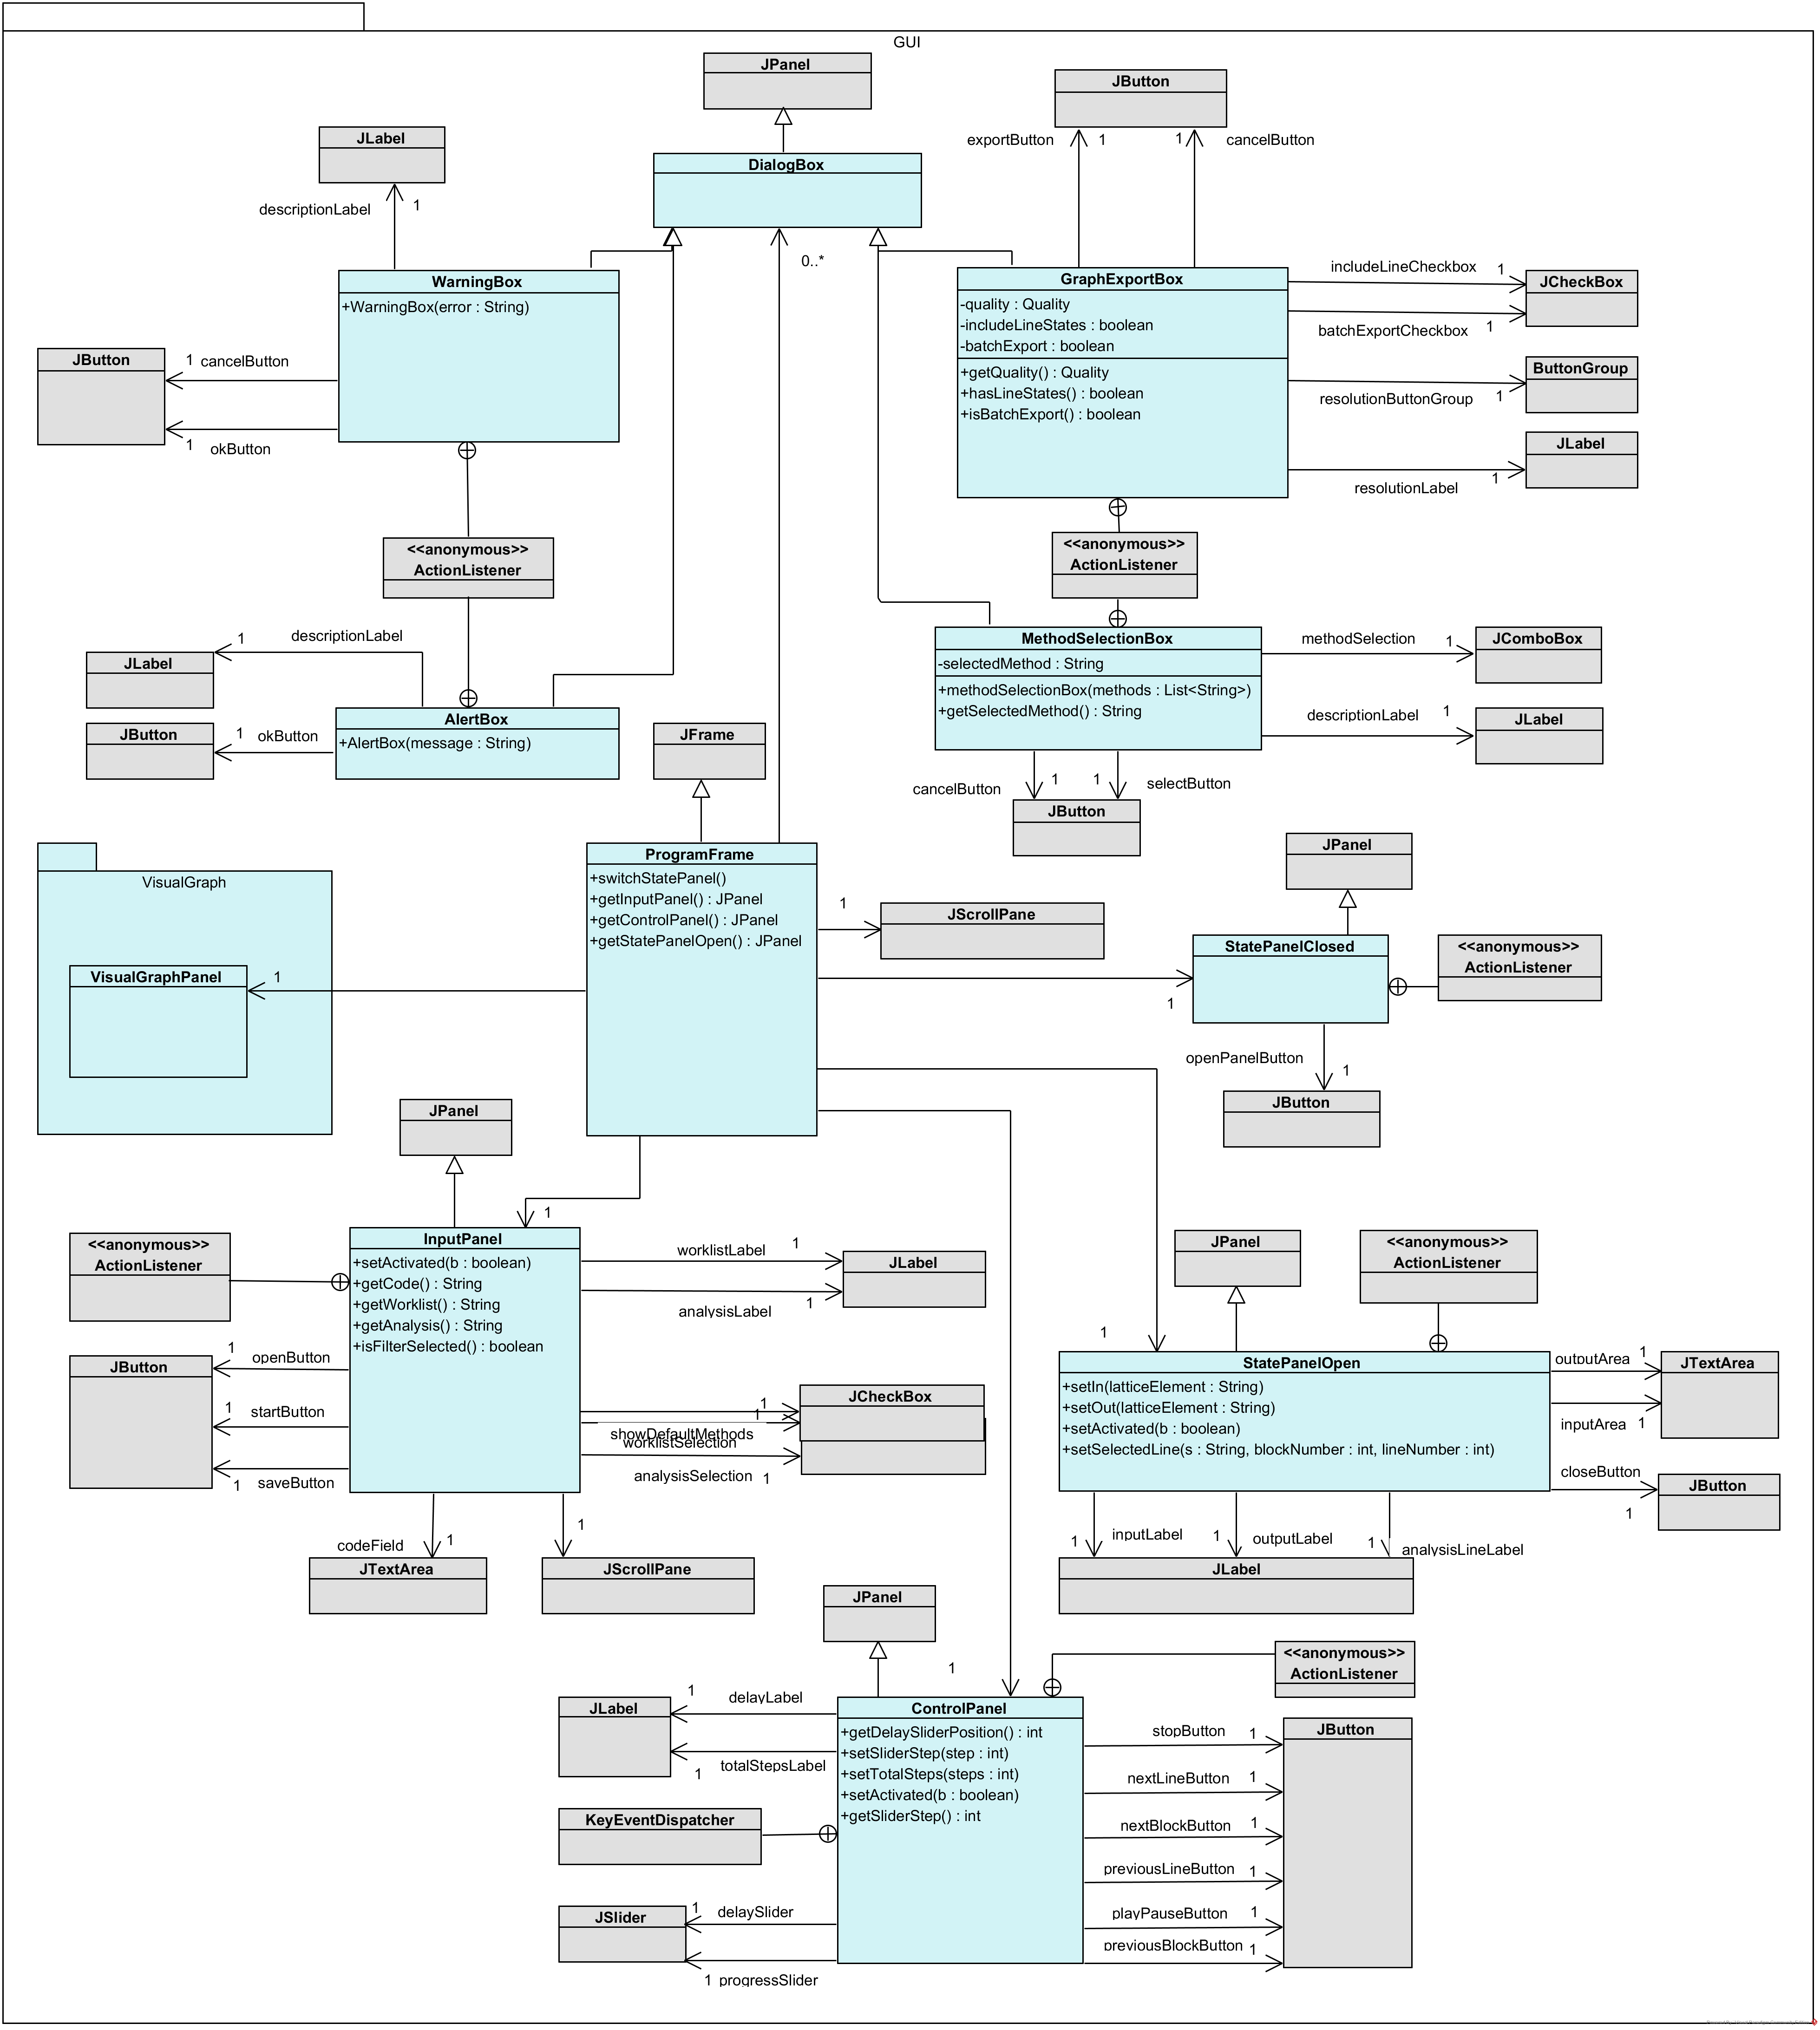
\includegraphics[width=1\textwidth]{Klassenuebersicht/GUI/GUI}
  \caption{Klassendiagramm des User Interfaces}
  \label{fig:UI}
\end{figure}

Das User Interface bildet die zentrale Schnittstelle für die Interaktion mit dem Benutzer.
Es ist aus vier zentralen Panels aufgebaut. 
Das \inlinecode{InputPanel} stellt die für den Benutzer notwendige Funktion für das Einlesen von Code, das Auswählen der Analyse oder des Worklist-Algorithmus und das Starten der Analyse zur Verfügung. 
Nach dem Starten der Analyse kann der Benutzer über das \inlinecode{ControlPanel} die Animation seiner Analyse kontrollieren. 
Die Änderungen, die sich dadurch am Graphen ergeben, werden im \inlinecode{VisualGraphPanel} angezeigt. 
Dieses ist in ein eigenes Modul, welches sich nur um die Visualisierung des Graphen in den verschiedenen Zuständen und um die Interaktion mit dem DFAFramework kümmert, ausgelagert. 
Das \inlinecode{StatePanel} zeigt die In- und Out-States der ausgewählten Zeile oder des ausgewählten Blocks an. 
Des Weiteren wird hier der Aufbau von vier verschiedenen \inlinecode{DialogBoxes} beschrieben. Diese dienen dazu, den Graph zu exportieren, zu analysierende Methoden auszuwählen und den Benutzer zu warnen oder über Fehler zu informieren. 

\subsubsection{Klassenbeschreibung}


\paragraph{ProgramFrame} $\;$ \\
\textbf{extends:} JFrame

\subparagraph{Attribute}
\begin{itemize}
	\item \attr{InputPanel}{JPanel}{private}{
		Panel, welches für die Eingabe des zu analysierenden Codes und für die Auswahl von Analyseart und Worklistalgorithmus verantwortlich ist.
	}
	\item \attr{ControlPanel}{JPanel}{private}{
		Panel, über welches der Benutzer die Animation während der Analyse des Codes steuern kann.
	}
	\item \attr{StatePanelOpen}{JPanel}{private}{
		Panel, in welchem dem Benutzer Informationen über die In- und Out-States des ausgewählten Blocks angezeigt werden.
	}
	\item \attr{StatePanelClosed}{JPanel}{private}{
		Panel, welches dargestellt wird, falls das StatePanel ausgeblendet wurde.
	}
	\item \attr{VisualGraphPanel}{JPanel}{private}{
		Panel, in welchem der Kontrollflussgraph dargestellt wird.
	}
\end{itemize}


\subparagraph{Methoden}
\begin{itemize}
	\item \method{switchStatePanel}{void}{}{public}{
		Macht entweder das StatePanelOpen, in dem die In- und Out-Informationen gegeben werden sichtbar und blendet StatePanelClosed aus oder blendet StatePanelOpen aus und blendet StatePanelClosed ein. 
	}
	\item \method{getInputPanel}{JPanel}{}{public}{
	Gibt das InputPanel zurück.
	}
	\item \method{getControlPanel}{JPanel}{}{public}{
	Gibt das ControlPanel zurück.
	}
	\item \method{getStatePanel}{JPanel}{}{public}{
	Gibt das StatePanelOpen zurück.
	}
\end{itemize}

\paragraph{InputPanel} $\;$ \\
\textbf{extends:} JPanel

\subparagraph{Attribute}
\begin{itemize}
	\item \attr{codeField}{JTextArea}{private}{
		Textfeld, in welchem der zu analysierende Code steht.
	}
	\item \attr{startButton}{JButton}{private}{
		Button, mit welchem der Benutzer die Analyse starten kann.
	}
	\item \attr{openButton}{JButton}{private}{
		Button, mit welchem der Benutzer eine .java-Datei aus seinem Dateisystem öffnen kann.
	}
	\item \attr{saveButton}{JButton}{private}{
		Button, mit welchem der angezeigte Code als .java-Datei gespeichert werden kann.
	}
	\item \attr{worklistLabel}{JLabel}{private}{
		Label, auf welchem steht, dass im Folgenden der Worklistalgorithmus ausgewählt werden kann.
	}
	\item \attr{analysisLabel}{JLabel}{private}{
		Label, auf welchem steht, dass im Folgenden die Analyse ausgewählt werden kann.
	}
	\item \attr{showDefaultMethods}{JCheckBox}{private}{
		Checkbox, durch welche bestimmt wird, ob Standardmethoden in der Methodenauswahl zur Verfügung stehen.
	}
	\item \attr{worklistSelection}{JComboBox}{private}{
		In dieser Auswahl kann der Worklistalgorithmus bestimmt werden.
	}
	\item \attr{analysisSelection}{JComboBox}{private}{
		In dieser Auswahl kann die Analyse ausgewählt werden.
	}
\end{itemize}


\subparagraph{Methoden}
\begin{itemize}
	\item \method{setActivated}{void}{active : boolean}{public}{
		Bestimmt, ob das InputPanel gerade verwendet werden kann oder nicht. Läuft eine aktuelle Analyse, ist das InputPanel deaktiviert und wird erst beim Abbruch der aktuellen Analyse wieder aktiv.
	}
	\item \method{getCode}{String}{}{public}{
		Gibt den aktuell angezeigten Java-Code zurück.
	}
	\item \method{getWorklist}{String}{}{public}{
		Gibt den Namen des aktuell ausgewählten Worklist-Algorithmus zurück.
	}
	\item \method{getAnalysis}{String}{}{public}{
		Gibt den Namen der aktuell ausgewählten Analyse zurück.
	}
	\item \method{isFilterSelected}{boolean}{}{public}{
		Gibt zurück, ob die Methoden gefiltert werden sollen oder nicht.
	}
\end{itemize}


\paragraph{ControlPanel} $\;$ \\
\textbf{extends:} JPanel

\subparagraph{Attribute}
\begin{itemize}
	\item \attr{delaySlider}{JSlider}{private}{
		Slider, mit welchem das Delay beim automatischen Durchlaufen der Analyse bestimmt werden kann.
	}
	\item \attr{progressSlider}{JSlider}{private}{
		Slider, mit welchem der Schritt der Analyse ausgewählt werden kann.
	}
	\item \attr{stopButton}{JButton}{private}{
		Button, mit welchem die Analyse abgebrochen werden kann.
	}
	\item \attr{nextLineButton}{JButton}{private}{
		Button, durch welchen die nächste Zeile im Graphen analysiert und die Darstellung dementsprechend geändert wird.
	}
	\item \attr{nextBlockButton}{JButton}{private}{
		Button, durch welchen der nächste Block im Graphen analysiert und die Darstellung dementsprechend geändert wird.
	}
	\item \attr{previousLineButton}{JButton}{private}{
		Button, durch welchen zum Zustand der Analyse in der vorherigen Zeile zurückgekehrt wird.
	}
	\item \attr{previousBlockButton}{JButton}{private}{
		Button, durch welchen zum Zustand der Analyse im vorherigen Block zurückgekehrt wird.
	}
	\item \attr{playPauseButton}{JButton}{private}{
		Button, mit welchem die automatische Wiedergabe der Analyse gestartet und pausiert werden kann.
	}
	\item \attr{totalStepsLabel}{JLabel}{private}{
		Label, auf welchem die Gesamtanzahl der Schritte der Analyse steht.
	}
	\item \attr{delayLabel}{JLabel}{private}{
		Label, durch welches der DelaySlider beschriftet wird.
	}
\end{itemize}


\subparagraph{Methoden}
\begin{itemize}
	\item \method{getDelaySliderPosition}{int}{}{public}{
		Gibt die Position des DelaySliders zurück.
	}
	\item \method{setSliderStep}{void}{step : int}{public}{
		Setzt die Position des StepSliders an den übergebenen Schritt.
	}
	\item \method{getSliderStep}{int}{}{public}{
		Gibt die Position des StepSliders zurück.
	}
	\item \method{setTotalSteps}{void}{steps: int}{public}{
		Schreibt die Gesamtanzahl der Schritte, die die Analyse macht, in das totalStepsLabel.
	}
	\item \method{setActivated}{void}{active: boolean}{public}{
		Bestimmt, ob das ControlPanel gerade verwendet werden kann oder nicht. Läuft eine aktuelle Analyse, ist das ControlPanel aktiviert und wird erst beim Abbruch der aktuellen Analyse deaktiviert.	
		}
\end{itemize}


\paragraph{StatePanelOpen} $\;$ \\
\textbf{extends:} JPanel

\subparagraph{Attribute}
\begin{itemize}
	\item \attr{analysisLineLabel}{JLabel}{private}{
		Label, auf welchem steht, an welcher Position sich die Analyse befindet.
	}
	\item \attr{inputLabel}{JLabel}{private}{
		Label, durch welches der Beginn der inputArea angezeigt wird.
	}
	\item \attr{outputLabel}{JLabel}{private}{
		Label, durch welches der Beginn der outputArea angezeigt wird.
	}
	\item \attr{inputArea}{JTextArea}{private}{
		Textfeld, in welcher der In-State der aktuell ausgewählten Komponente steht.
	}
	\item \attr{outputArea}{JTextArea}{private}{
		Textfeld, in welcher der out-State der aktuell ausgewählten Komponente steht.
	}
	\item \attr{closeButton}{JButton}{private}{
		Button, mit welchem das StatePanel geschlossen werden kann.
	}
\end{itemize}


\subparagraph{Methoden}
\begin{itemize}
	\item \method{setIn}{void}{latticeElement : String}{public}{
		Zeigt die Text-Repräsentation des übergebenen LatticeElements für in den In-State in dem entsprechenden Textfeld an.
	}
	\item \method{setOut}{void}{latticeElement : String}{public}{
		Zeigt die Text-Repräsentation des übergebenen LatticeElements für in den Out-State in dem entsprechenden Textfeld an.
	}
	\item \method{setSelectedLine}{void}{content : String, blockNumber : int, lineNumber : int}{public}{
		Zeigt die Text-Repräsentation des ausgewählten Blocks oder der ausgewählten Zeile im entsprechenden Textfeld an und fügt die Nummer des Blockes oder der Zeile hinzu.
	}
	\item \method{setActivated}{void}{active : boolean}{public}{
		Bestimmt, ob das StatePanelOpen gerade verwendet werden kann oder nicht. Läuft eine aktuelle Analyse, ist das StatePanelOpen aktiviert und wird erst beim Abbruch der aktuellen Analyse wieder deaktiviert.
	}
\end{itemize}

\paragraph{StatePanelClose} $\;$ \\
\textbf{extends:} JPanel

\subparagraph{Attribute}
\begin{itemize}
	\item \attr{openPanelButton}{JButton}{private}{
		Button, mit welchem das StatePanelOpen geöffnet werden kann.
	}
\end{itemize}



\paragraph{DialogBox} $\;$ \\
\textbf{extends:} JPanel

\subparagraph{Attribute}
\begin{itemize}
	\item \attr{title}{String}{private}{
		Bestimmt den Titel der Dialogbox.
	}
\end{itemize}


\paragraph{MethodSelectionBox} $\;$ \\
\textbf{extends:} DialogBox

\subparagraph{Attribute}
\begin{itemize}
	\item \attr{selectedMethod}{String}{private}{
		String, in welchem die ausgewählte Methode gespeichert wird.
	}
	\item \attr{methodSelection}{JComboBox}{private}{
		ComboBox, in welcher alle Methoden aufgelistet sind und aus ihnen ausgewählt werden kann.
	}
	\item \attr{descriptionLabel}{JLabel}{private}{
		Label, in welchem erklärende Anweisungen gegeben werden.
	}
	\item \attr{cancelButton}{JButton}{private}{
		Button, mit welchem der Vorgang abgebrochen werden kann.
	}
	\item \attr{selectButton}{JButton}{private}{
		Button, mit welchem das Fenster geschlossen und die Methode endgültig ausgewählt werden kann.
	}
\end{itemize}


\subparagraph{Methoden}
\begin{itemize}
	\item \method{methodSelectionBox}{void}{methods : List<String>}{public}{
		Übergibt eine Liste von im Code vorhandenen Methoden, zwischen denen ausgewählt werden können soll.
	}
	\item \method{getSelectedMethod}{String}{}{public}{
		Gibt zurück, welche Methode aktuell ausgewählt ist.
	}
\end{itemize}


\paragraph{GraphExportBox} $\;$ \\
\textbf{extends:} DialogBox

\subparagraph{Attribute}
\begin{itemize}
	\item \attr{quality}{Quality}{private}{
		Legt die ausgewählte Qualität fest.
	}
	\item \attr{includeLineStates}{boolean}{private}{
		Gibt an, ob LineStates in den BatchExport integriert werden sollen.
	}
	\item \attr{batchExport}{boolean}{private}{
		Gibt an, ob BatchExport ausgewählt wurde.
	}
	\item \attr{batchExportCheckBox}{JCheckBox}{private}{
		CheckBox, in der ausgewählt wird, ob ein BatchExport durchgeführt wird.
	}
	\item \attr{includeLineCheckBox}{JCheckBox}{private}{
		CheckBox, in der ausgewählt wird, ob LineStates integriert werden.
	}
	\item \attr{resolutionButtonGroup}{ButtonGroup}{private}{
		Buttons, durch welche die Qualität bestimmt werden kann.
	}
	\item \attr{exportButton}{JButton}{private}{
		Button, mit welchem die Eingaben bestätigt und der Export durchgeführt werden kann.
	}
	\item \attr{cancelButton}{JButton}{private}{
		Button, mit welchem der Vorgang abgebrochen werden kann.
	}
	\item \attr{resolutionLabel}{JLabel}{private}{
		Label, das beschreibt, was im Folgenden gewählt werden kann.
	}
\end{itemize}


\subparagraph{Methoden}
\begin{itemize}
	\item \method{getQuality}{Quality}{}{public}{
		Gibt die ausgewählte Qualität zurück.
	}
	\item \method{hasLineStates}{boolean}{}{public}{
		Gibt zurück, ob die Zeilen in den BatchExport mit aufgenommen werden sollen.
	}
	\item \method{isBatchExport}{boolean}{}{public}{
		Gibt zurück, ob BatchExport ausgewählt wurde.
	}
\end{itemize}


\paragraph{WarningBox} $\;$ \\
\textbf{extends:} JPanel

\subparagraph{Attribute}
\begin{itemize}
	\item \attr{descriptionLabel}{JLabel}{private}{
		Label, in welchem der Fehler ausgegeben wird.
	}
	\item \attr{cancelButton}{JButton}{private}{
		Button, mit welchem der Vorgang abgebrochen werden kann.
	}
	\item \attr{okButton}{JButton}{private}{
		Button, damit der Vorgang trotzdem durchgeführt wird.
	}
\end{itemize}


\subparagraph{Konstruktoren}
\begin{itemize}
	\item \ctor{WarningBox}{message: String}{public}{
		Schreibt die entsprechende Nachricht in das Label.
	}
\end{itemize}


\paragraph{AlertBox} $\;$ \\
\textbf{extends:} DialogBox

\subparagraph{Attribute}
\begin{itemize}
	\item \attr{descriptionLabel}{JLabel}{private}{
		Label, in welchem die Fehlermeldung ausgegeben wird.
	}
	\item \attr{okButton}{JButton}{private}{
		Button, mit welchem sich das Fenster wieder schließt.
	}
\end{itemize}


\subparagraph{Konstruktoren}
\begin{itemize}
	\item \ctor{AlertBox}{error : String}{public}{
		Schreibt die entsprechende Nachricht in das Label.
	}
\end{itemize}
	%note: don't split this document up with include{...}

\section{VisualGraph}

\subsection{Klassendiagramm}

\begin{figure}[H]
\centering
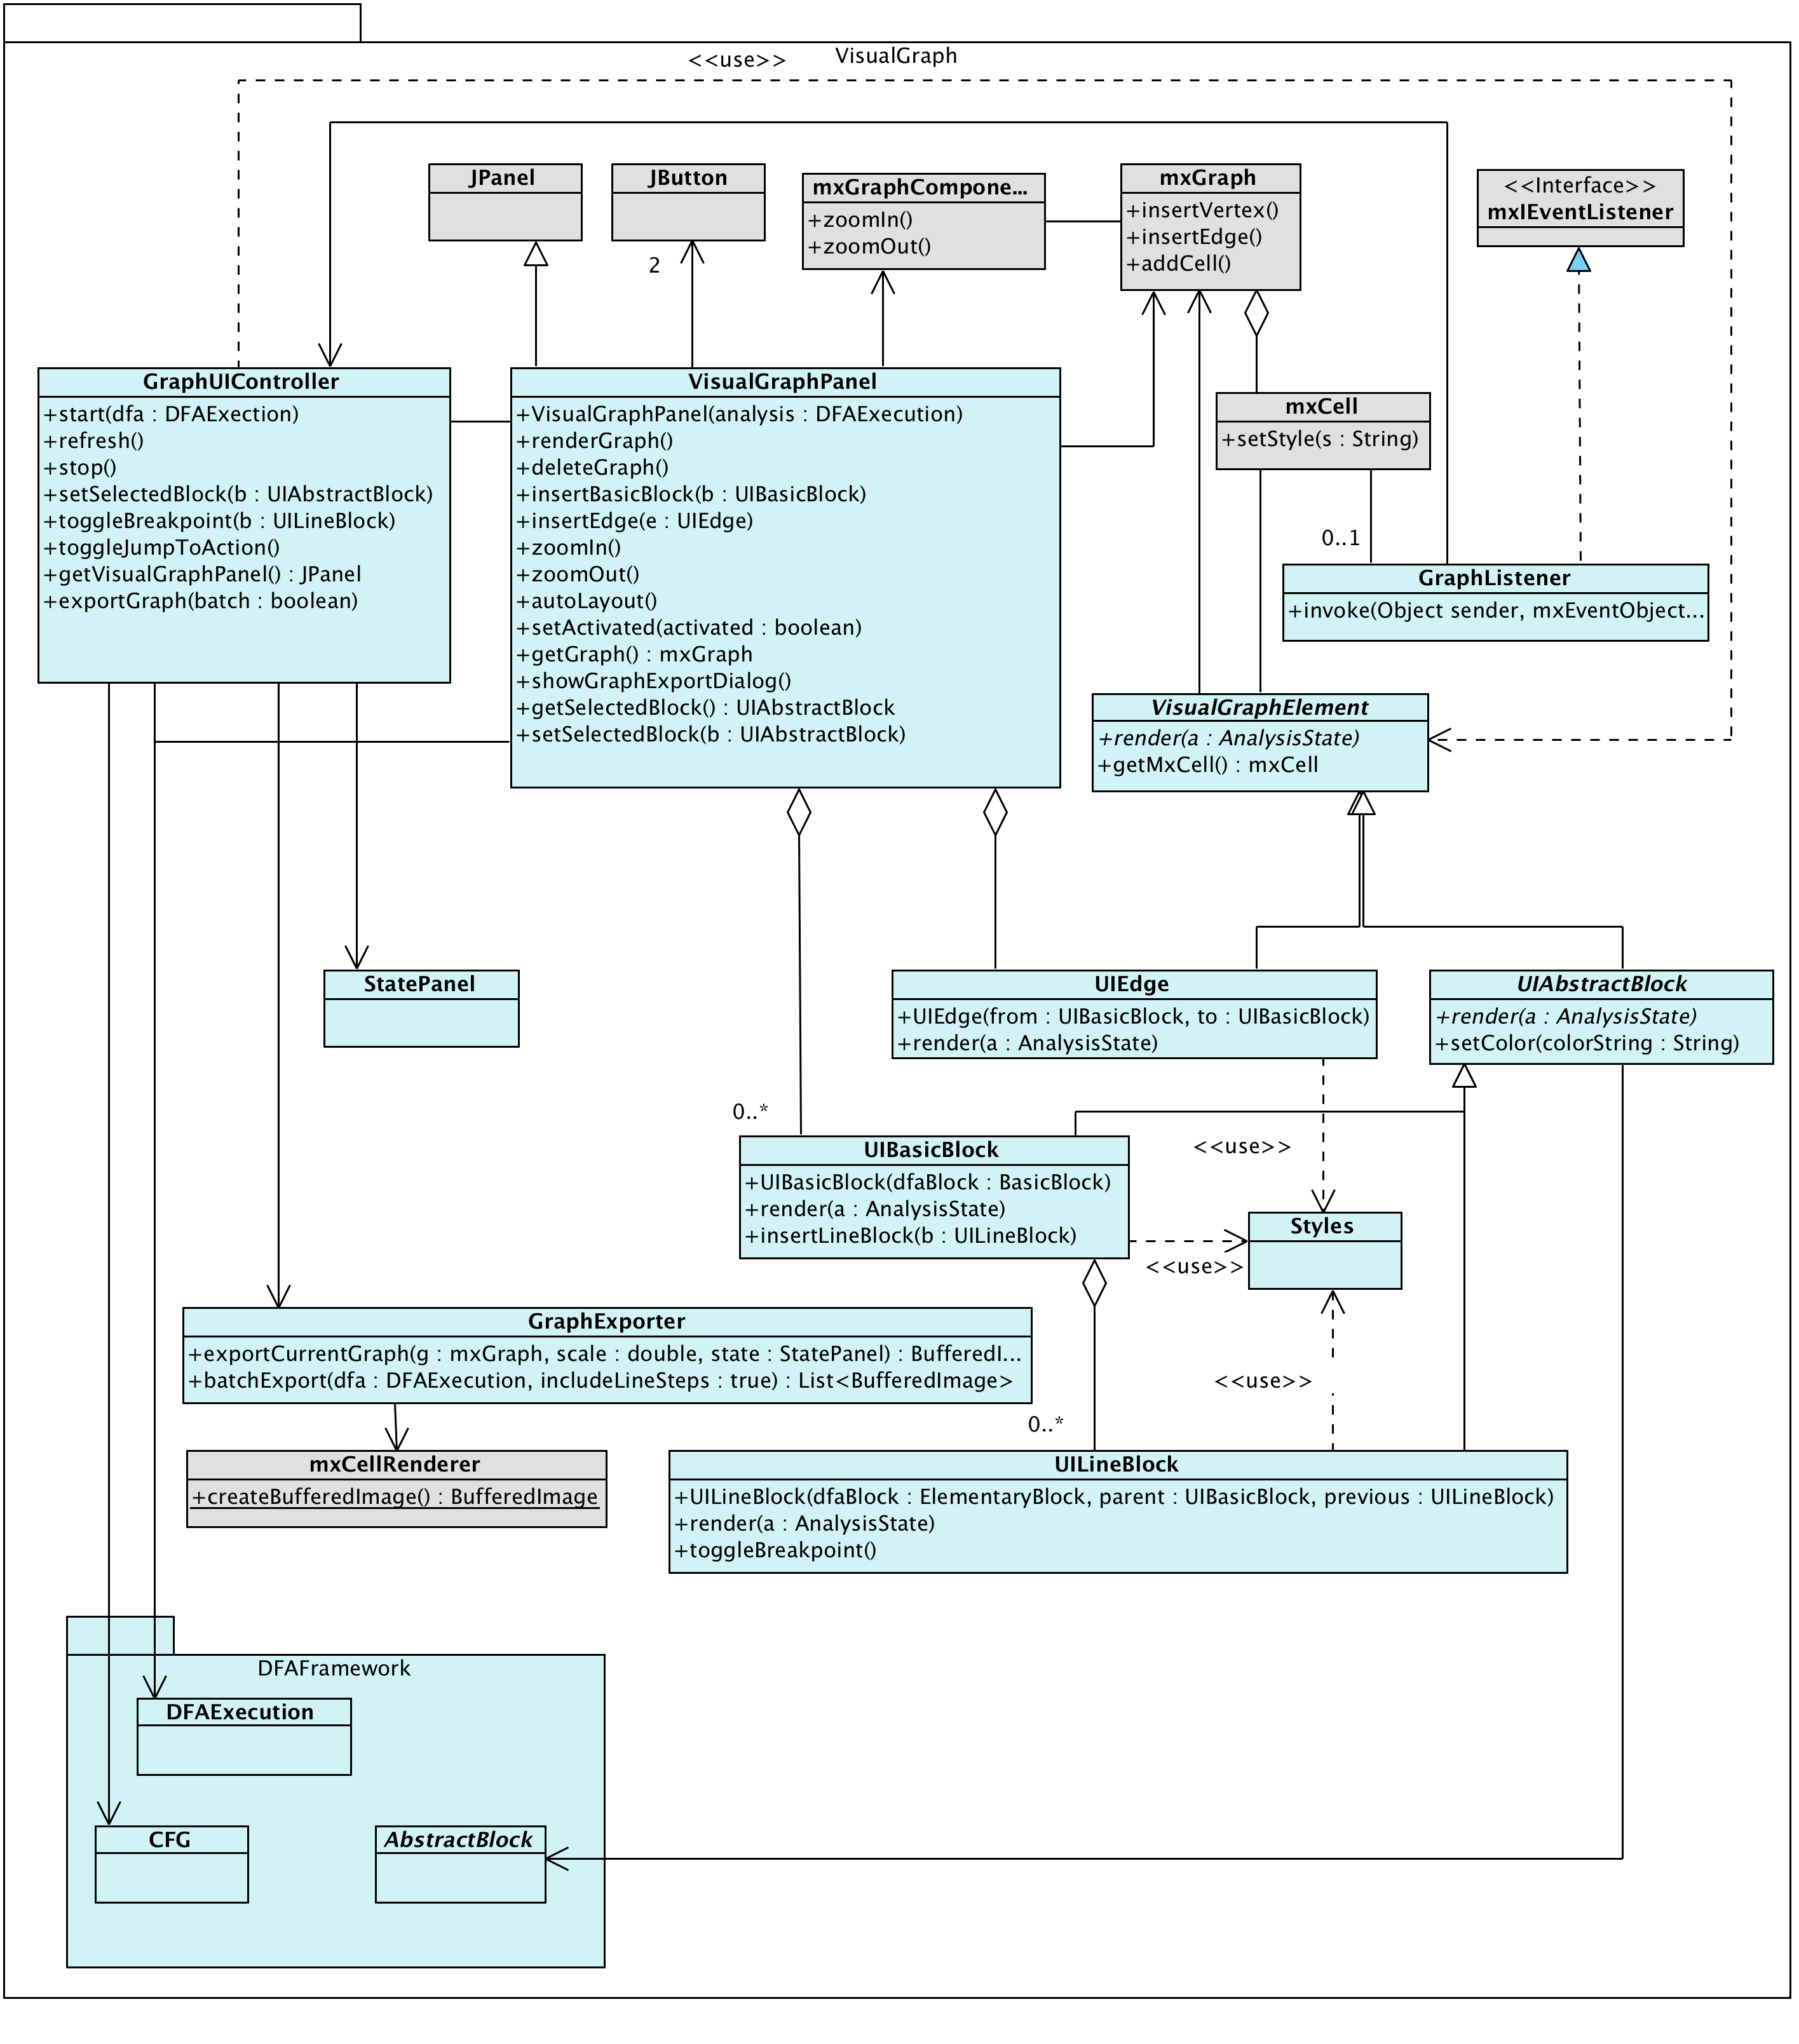
\includegraphics[width=1\textwidth]{Klassenuebersicht/VisualGraph/VisualGraph}
\end{figure}

\newpage

\subsection{Klassenbeschreibung}

Das VisualGraph-Modul ist dafür zuständig, aktuelle Daten aus dem DFAFramework abzufragen und diese visuell in einem Graphen darzustellen. 
Zusätzlich ermöglicht es dem Nutzer, Breakpoints für die Analyse zu setzen und den Graphen als PNG-Datei zu exportieren.

Als zentrale logische Schnittstelle bietet das VisualGraph-Modul die Klasse \inlinecode{GraphUIController}. 
Diese muss vom Controller-Modul über den Aufruf von start() oder refresh() darüber benachrichtigt werden, dass es Änderungen in der Analyse des DFAFrameworks gegeben hat.
Ist diese Benachrichtigung erfolgt, so beschafft sich der \inlinecode{GraphUIController} selbsttätig alle benötigten Daten vom DFAFramework, um die Objektstruktur für den visuellen Graphen zu erstellen und den Graphen zu rendern.

Die zweite nach außen wichtige Schnittstelle ist die Klasse \inlinecode{VisualGraphPanel}. Diese erbt von \inlinecode{JPanel} und beherbergt direkt den visuellen Graphen.
Zusätzlich stehen für die Visualisierung wichtige Methoden wie zoomIn(), zoomOut() und setActivated() zu Verfügung.
Die übrigen Methoden des \inlinecode{VisualGraphPanel}s werden ausschließlich von \inlinecode{GraphUIController}, \inlinecode{GraphExporter} und Listener-Objekten aufgerufen.

Bemerkenswert am Entwurf des VisualGraph-Moduls ist die Entkopplung der Visualisierungslogik von der benutzten Library JGraphX.
So arbeiten weder \inlinecode{VisualGraphPanel} noch \inlinecode{GraphUIController} direkt mit der Klasse \inlinecode{mxCell}, welche alle visuellen Komponenten in JGraphX repräsentiert.
Stattdessen wird auf eine eigene Struktur mit der Klasse \inlinecode{VisualGraphElement} und ihren Subklassen \inlinecode{UIEdge}, \inlinecode{UIAbstractBlock}, \inlinecode{UIBasicBlock} und \inlinecode{UILineBlock} gesetzt.
Jedes \inlinecode{VisualGraphElement} besitzt eine Referenz auf das \inlinecode{mxGraph}-Objekt, eine Referenz auf den zugehörigen logischen Block aus dem DFAFramework und eine render()-Methode.
Beim ersten Aufruf von render() wird nun dafür gesorgt, dass die entsprechende \inlinecode{mxCell} erstellt und in den \inlinecode{mxGraph} eingefügt wird.
Wird render() erneut auf dem selben Objekt aufgerufen, so aktualisiert es seine Daten, indem es diese beim DFAFramework abfragt.
Anschließend aktualisiert es seine zugehörige \inlinecode{mxCell}, um den angezeigten Graphen neu zu rendern.

Für den Entwurf ergeben sich folgende Vorteile:
\begin{itemize}
	\item Die Klassen \inlinecode{GraphUIController} und \inlinecode{VisualGraphPanel} müssen sich nicht mit Layouts, Größen oder Koordinaten auseinandersetzen, da dies von den \inlinecode{VisualGraphElement}-Subklassen erledigt wird.
	    Die Erstellung eines visuellen Grundblocks mit JGraphX ist komplex (für jede Zeile eines Grundblocks wird eine eigene verschachtelte \inlinecode{mxCell} benötigt, und Zeilen müssen alle untereinander gerendert werden).
	    Durch die gegebene Entwurfsarchitektur wird diese Komplexität versteckt, sodass der visuelle Graph sehr einfach erstellt werden kann.
	\item Durch die Entkopplung wird ein Austausch von JGraphX stark erleichtert, da in diesem Fall hauptsächlich die Subklassen von \inlinecode{VisualGraphElement} geändert werden müssen.
        Das \inlinecode{VisualGraphPanel} hat zwar ebenfalls eine Referenz auf \inlinecode{mxGraph}, allerdings nur, um diesen in den \inlinecode{mxGraphComponent} einzufügen. 
        Auch die getGraph()-Methode im \inlinecode{VisualGraphPanel} ist nur für den Batch-Export notwendig.
        Abgesehen davon wäre es also ausreichend, die Subklassen von \inlinecode{VisualGraphElement} und wenige Zeilen im \inlinecode{VisualGraphPanel} zu ändern, um JGraphX gegen eine andere Library auszutauschen.
        
\end{itemize}

% the template for one class description

\class{VisualGraphPanel extends JPanel}

Das Panel, welches den visuellen Graphen sowie Jump-to-Action- und Graph-Export-Button enthält. 
Es besitzt außerdem Methoden, um Blöcke und Kanten einzufügen, den Graphen zu rendern und zu zoomen.

\subparagraph{Konstruktoren} % skip this if there are no constructors
\begin{itemize}
	\item \ctor{VisualGraphPanel}{analysis: DFAExecution}{public}{
		Erstellt ein neues \inlinecode{VisualGraphPanel}, welches auf der gegebenen \inlinecode{DFAExecution} operiert.
	}
\end{itemize}

\subparagraph{Methoden}  % skip this if there are no methods
\begin{itemize}
	\item \method{renderGraph}{void}{}{public}{
		Erstellt bzw. aktualisiert den visuellen \inlinecode{mxGraph}-Graphen und macht diesen sichtbar.
		Dies geschieht durch Aufruf von render() auf allen hinzugefügten \inlinecode{VisualGraphElement}s.
	}
	\item \method{deleteGraph}{void}{}{public}{
		Entfernt den \inlinecode{mxGraph}-Graphen aus dem Panel und löscht ihn.
	}
	\item \method{insertBasicBlock}{void}{b: UIBasicBlock}{public}{
		Fügt den gegebenen \inlinecode{UIBasicBlock} ein, sodass dieser beim nächsten Aufruf von renderGraph() angezeigt wird.
	}
	\item \method{insertEdge}{void}{e: UIEdge}{public}{
		Fügt die gegebene \inlinecode{UIEdge} ein, sodass diese beim nächsten Aufruf von renderGraph() angezeigt wird.
	}
	\item \method{zoomIn}{void}{}{public}{
		Zoomt in den Graphen hinein durch Aufruf von \inlinecode{mxGraphComponent}.zoomIn().
	}
	\item \method{methodName}{void}{}{public}{
		Zoomt aus dem Graphen heraus durch Aufruf von \inlinecode{mxGraphComponent}.zoomOut().
	}
	\item \method{autoLayout}{void}{}{public}{
		Führt den Auto-Layouter auf dem angezeigten Graphen aus.
	}
	\item \method{setActivated}{void}{isActivated: boolean}{public}{
		Legt fest, ob das VisualGraphPanel Benutzerinteraktion ermöglichen soll.
	}
	\item \method{getGraph}{mxGraph}{}{public}{
        Gibt den \inlinecode{mxGraph} zurück. Diese Methode wird für den Graph-Export benötigt.
	}
	\item \method{setCurrentBlock}{void}{b: UIAbstractBlock}{public}{
		Setzt den aktuellen Block der Analyse. 
		Diese Methode wird beim Aufruf von render() eines \inlinecode{UIAbstractBlock}s aufgerufen, falls der entsprechende Block des DFAFrameworks gerade der aktuelle Block der Analyse ist.
		So wird gewährleistet, dass das \inlinecode{VisualGraphPanel} den aktuellen \inlinecode{UIAbstractBlock} kennt und die Jump-to-Action-Funktion benutzt werden kann.
	}
	\newpage
	\item \method{getSelectedBlock}{void}{}{UIAbstractBlock}{
		Gibt den \inlinecode{UIAbstractBlock}, der dem aktuellen Block aus der Analyse des DFAFrameworks entspricht, zurück.
		Diese Methode wird für die Jump-to-Action-Funktion benötigt und vom \inlinecode{GraphUIController} aufgerufen.
	}
	\item \method{showGraphExportDialog}{void}{}{public}{
		Zeigt den Graph-Export-Dialog an.
	}
\end{itemize}

\class{GraphUIController}
Der \inlinecode{GraphUIController} ist dafür zuständig, das \inlinecode{VisualGraphPanel} zu erstellen und die \inlinecode{VisualGraphElement}s darin einzufügen. 
Dazu bietet er die zentralen Methoden start(), update() und stop().
Diese werden vom Controller-Modul aufgerufen, sobald sich eine Änderung der Analyse des DFAFrameworks ergeben hat.

\subparagraph{Konstruktoren} % skip this if there are no constructors
\begin{itemize}
	\item \ctor{GraphUIController}{}{public}{
	    Erstellt einen neuen \inlinecode{GraphUIController} und ein zugehöriges \inlinecode{VisualGraphPanel}.
	}
\end{itemize}

\subparagraph{Methoden}  % skip this if there are no methods
\begin{itemize}
	\item \method{start}{void}{dfa: DFAExecution}{public}{
		Wird vom Controller nach Analysestart aufgerufen. 
		Durch diese Methode werden alle benötigten Daten vom DFAFramework abgerufen.
		Anschließend werden die \inlinecode{VisualGraphElement}s erstellt und in das \inlinecode{VisualGraphPanel} eingefügt.
		Danach wird renderGraph() auf dem \inlinecode{VisualGraphPanel} aufgerufen, um den Graphen anzuzeigen.
		Zuletzt wird autoLayout() auf dem \inlinecode{VisualGraphPanel} aufgerufen.
	}
	\item \method{refresh}{void}{}{public}{
		Wird vom Controller nach jedem Analyseschritt aufgerufen.
		Diese Methode ruft renderGraph() erneut auf, ohne autoLayout() auszuführen.
		Der angezeigte Graph wird dadurch aktualisiert. 
	}
	\item \method{stop}{void}{}{public}{
		Entfernt und löscht den angezeigten Graphen durch Aufruf von deleteGraph() auf dem \inlinecode{VisualGraphPanel}.
	}
	\item \method{setSelectedBlock}{void}{b: UIAbstractBlock}{public}{
		Setzt den aktuell ausgewählten Block durch Aufruf von setSelected() auf dem entsprechenden \inlinecode{UIAbstractBlock}.
	}
	\item \method{toggleBreakpoint}{void}{b: UILineBlock}{public}{
		Setzt bzw. entfernt einen Breakpoint durch Aufruf von toggleBreakpoint() auf dem entsprechenden \inlinecode{UILineBlock}.
	}
	\item \method{toggleJumpToAction}{void}{}{public}{
		Aktiviert bzw. deaktiviert die Jump-to-Action-Funktion. 
		Falls diese aktiviert ist, wird bei jedem Aufruf von refresh() der ausgewählte Block auf den aktuellen Block der Analyse gesetzt (durch Aufruf von setSelectedBlock())
	}
	\item \method{getVisualGraphPanel}{VisualGraphPanel}{}{public}{
		Gibt das \inlinecode{VisualGraphPanel} zurück.
		Diese Methode wird benötigt, um das Panel in das \inlinecode{ProgramFrame} einfügen zu können.
	}
	\item \method{exportGraph}{void}{batch: boolean}{public}{
		Erstellt einen neuen \inlinecode{GraphExporter} und führt den Export durch Aufruf von exportCurrentGraph() bzw. batchExport() auf dem \inlinecode{GraphExporter} durch.
	}
\end{itemize}

% the template for one class description

\class{abstract VisualGraphElement}
%Brief descrition of SomeClass.

\subparagraph{Methoden}  % skip this if there are no methods
\begin{itemize}
	\item \method{render}{void}{a: AnalysisState}{public abstract}{
		Erstellt eine (je nach Subklasse unterschiedliche) \inlinecode{mxCell} und fügt diese in das \inlinecode{mxGraph}-Objekt ein.
		Falls die \inlinecode{mxCell} bereits existiert, so wird diese mit den aktuellen Daten des entsprechenden Blocks des DFAFrameworks aktualisiert.
	}
	\item \method{getMxCell}{mxCell}{}{public}{
		Gibt die zugehörige mxCell zurück.
		Wird in der render()-Methoden des \inlinecode{UILineBlock}s und der \inlinecode{UIEdge} benötigt.
	}
\end{itemize}

\class{UIEdge extends VisualGraphElement}
Die Repräsentation einer Kante im visuellen Graphen.

\subparagraph{Konstruktoren} % skip this if there are no constructors
\begin{itemize}
	\item \ctor{UIEdge}{from: UIBasicBlock, to: UIBasicBlock}{public}{
		Erstellt eine neue \inlinecode{UIEdge} zwischen den entsprechenden \inlinecode{UIBasicBlock}s.
	}
\end{itemize}

\subparagraph{Methoden}  % skip this if there are no methods
\begin{itemize}
	\item \method{render}{void}{a: AnalysisState}{public}{
		Erstellt eine Kante im mxGraph-Objekt.
		Die im Konstruktor übergebenen \inlinecode{UIBasicBlock}s müssen bereits gerendert sein, damit die \inlinecode{UIEdge} erfolgreich gerendert werden kann.
	}
\end{itemize}

\class{abstract UIAbstractBlock extends VisualGraphElement}
Die Repräsentation eines Blockes (Parent- oder Zeilenblock) im visuellen Graphen.

\subparagraph{Methoden}  % skip this if there are no methods
\begin{itemize}
	\item \method{setSelected}{void}{isSelected: boolean}{public}{
		Bestimmt, ob die zugehörige \inlinecode{mxCell} ausgewählt sein soll.
	}
\end{itemize}

\newpage
\class{UIBasicBlock}
Die Repräsentation eines BasicBlocks im visuellen Graphen.

\subparagraph{Konstruktoren} % skip this if there are no constructors
\begin{itemize}
	\item \ctor{UIBasicBlock}{dfaBlock: BasicBlock}{public}{
		Erstellt einen neuen \inlinecode{UIBasicBlock}, welcher dem übergebenen \inlinecode{BasicBlock} entspricht.
	}
\end{itemize}

\subparagraph{Methoden}  % skip this if there are no methods
\begin{itemize}
	\item \method{render}{void}{a: AnalysisState}{public}{
		Erstellt einen Grundblock im \inlinecode{mxGraph}-Objekt und ruft render() auf allen zugehörigen \inlinecode{UILineBlock}s auf.
	}
	\item \method{insertLineBlock}{void}{b: UILineBlock}{public}{
		Fügt einen \inlinecode{UILineBlock} in den \inlinecode{UIBasicBlock} ein.
	}
\end{itemize}

\class{UILineBlock}
Die Repräsentation eines \inlinecode{ElementaryBlock}s im visuellen Graphen.

\subparagraph{Konstruktoren} % skip this if there are no constructors
\begin{itemize}
	\item \ctor{UILineBlock}{dfaBlock: ElementaryBlock, parent: UIBasicBlock, previous: UILineBlock}{public}{
		Erstellt einen neuen \inlinecode{UILineBlock}, der dem übergebenen \inlinecode{ElementaryBlock} entspricht.
	}
\end{itemize}

\subparagraph{Methoden}  % skip this if there are no methods
\begin{itemize}
	\item \method{render}{void}{a: AnalysisState}{public}{
		Erstellt eine Zeile in der Parent-\inlinecode{mxCell} und zeigt diese an.
	}
	\item \method{toggleBreakpoint}{void}{}{public}{
		Aktiviert bzw. deaktiviert die Anzeige eines Breakpoints in der Zeile.
	}
\end{itemize}

\class{GraphListener implements mxIEventListener}
Jede \inlinecode{mxCell} besitzt einen eigenen \inlinecode{GraphListener}, der Click-Events verarbeitet, um Methoden auf dem \inlinecode{GraphUIController} aufzurufen.

\subparagraph{Methoden}  % skip this if there are no methods
\begin{itemize}
	\item \method{invoke}{void}{sender: Object, evt: mxEventObject}{public}{
		Wird aufgerufen, wenn der Nutzer die zugehörige \inlinecode{mxCell} aufgerufen hat.
		Diese Methode ruft die dem Event entsprechende Methode des \inlinecode{GraphUIController}s auf.
	}
\end{itemize}

\class{Styles}

Diese Klasse besitzt Konstanten für die visuelle Anzeige des Graphen. 
Diese sind \inlinecode{mxGraph}-Style-Strings und Zahlenwerte, welche die Maße der Blöcke festlegen.

\class{GraphExporter}
Diese Klasse ist für den Graph-Export zuständig. Dies beinhaltet den Export des aktuellen Zustandes sowie den Batch-Export aller Zustände.

\subparagraph{Methoden}  % skip this if there are no methods
\begin{itemize}
	\item \method{exportCurrentGraph}{BufferedImage}{g: mxGraph, scale: double, state: StatePanel}{public}{
		Exportiert den aktuellen Graphen und eine Visualisierung des \inlinecode{StatePanel}s als Bild.
	}
	\item \method{batchExport}{BufferedImage}{dfa: DFAExecution, includeLineSteps: boolean}{public}{
		Führt einen Batch-Export aller Analyse-Zustände durch.
		Dabei wird mithilfe der übergebenen DFAExecution ein neuer \inlinecode{GraphUIController} und ein neues \inlinecode{VisualGraphPanel} mitsamt \inlinecode{mxGraph} erstellt.
		Dadurch wird die angezeigte Analyse durch den Batch-Export nicht beeinflusst.
		Mit den erstellten Objekten wird die Analyse dann vollständig durchgelaufen.
		Dabei wird nach jedem Schritt der Analyse der Graph mitsamt In- und Out-States durch Aufruf von exportCurrentGraph() als Bild exportiert.
	}
\end{itemize}

	%note: don't split this document up with include{...}

\section{GraphExport}

	%note: don't split this document up with include{...}

\section{Sequenzdiagramme}
	\part{Nachträgliche Änderungen am Pflichtenheft}

\subsection*{Unterstütztes Java-Subset} 
Da jede Analyse mit (Jimple-)Statements auf eine eigene Art und Weise umgeht, ist in jeder implementierten Analyse der Umgang mit den Statements einzeln definiert.
Dies bedeutet, dass alle im Pflichtenheft angegebenen Kontrollflussstrukturen und Statements für alle im Pflichtenheft angegebenen Analysen implementiert werden.
Falls ein Endbenutzer sich dazu entschließt selbst eine Analyse zu erstellen, so muss er selbst festlegen mit welchen Statements seine Analyse funktionieren soll und den Umgang mit diesen implementieren.
Stößt das Programm bei der Durchführung der Analyse auf ein Statement für welches kein Verhalten festgelegt wurde, so wird eine Fehlermeldung erzeugt.
	\part{Klassendiagramm}
\begin{figure}[H]
	\centering
	\includegraphics[width=1\textwidth]{Klassendiagramm/completeOverview}
	\caption{Gesamtes Klassendiagramm}
	\label{fig:start}
\end{figure}

\end{document}